\documentclass[11pt,a4paper]{article}

% Schnelle Overleaf-Version: bewusst ohne TikZ/tcolorbox und ohne biblatex/Biber.
% Die Literaturdatei muss im selben Overleaf-Projekt liegen und exakt
% "Protokoll_Vibrating_Reed_Literatur.bib" heißen.
\RequirePackage[skip = 0.5\baselineskip plus 2pt]{parskip}

\usepackage[ngerman]{babel}
\usepackage[utf8]{inputenc}
\usepackage[T1]{fontenc}
\usepackage[a4paper,margin=1in]{geometry}
\usepackage{graphicx}
\usepackage{mathtools}
\usepackage{amssymb}
\DeclarePairedDelimiterX{\set}[2]{\lbrace}{\rbrace}{#1 \;\delimsize\vert\; \mathopen{} #2} % \delimsize is the size of the outer delimiters

\usepackage{siunitx}
\DeclareSIUnit{\rad}{rad}
\sisetup{locale=DE,separate-uncertainty=true}
\usepackage{booktabs,array,longtable,tabularx}
\usepackage{arraycols}
\usepackage{float}
\usepackage{xcolor}
\usepackage{enumitem}
\usepackage{listings}
\usepackage{csquotes}
\usepackage{subcaption}
\usepackage{todonotes}
\usepackage{placeins}
\usepackage[style=numeric,url=true]{biblatex}
\addbibresource{bibliography.bib}                     
\usepackage{zref-clever}
\usepackage[colorlinks=true,linkcolor=blue,citecolor=blue,urlcolor=blue]{hyperref}

\definecolor{resultorange}{RGB}{210,105,0}
\definecolor{lightblue}{RGB}{242,247,252}
\definecolor{lightorange}{RGB}{255,248,238}
\definecolor{lightgray}{RGB}{247,247,247}
\definecolor{libarygreen}{RGB}{56, 172, 148}% {78,201,176}

\newcommand{\libary}[1]{\textcolor{libarygreen}{\texttt{\detokenize{#1}}}}

\lstdefinestyle{mypython}{
  basicstyle=\ttfamily\footnotesize,
  breaklines=true,
  frame=single,
  numbers=left,
  numberstyle=\tiny,
  showstringspaces=false,
  tabsize=4
}
\lstdefinestyle{mylabview}{
  basicstyle=\ttfamily\footnotesize,
  breaklines=true,
  frame=single,
  numbers=none,
  showstringspaces=false
}

% Orange Inhalte werden später vollständig durch reale Ergebnisse ersetzt.
\newcommand{\messfeld}[1][3cm]{\textcolor{resultorange}{\textit{Messwert einsetzen}}}
\newcommand{\platzhalter}[1]{\textcolor{resultorange}{\textit{[#1]}}}
\newcommand{\erwartung}[1]{\textcolor{resultorange}{#1}}
\newcommand{\ersatztext}[1]{\textcolor{resultorange}{\textit{#1}}}
\newcommand{\checkitem}{\(\square\)}
\newcommand{\eintrag}[2][3.5cm]{\textbf{#2:} \rule{#1}{0.4pt}}

\renewcommand{\arraystretch}{1.25}
\setlist[enumerate]{itemsep=0.35em,topsep=0.4em}
\setlist[itemize]{itemsep=0.25em,topsep=0.35em}

% Leichtgewichtige Hervorhebungen statt tcolorbox/TikZ.
\newenvironment{aufgabenbox}[1]{%
  \par\medskip\noindent\colorbox{lightblue}{\parbox{0.965\linewidth}{\textbf{#1}}}\par\smallskip
  \begin{quote}}
 {\end{quote}\medskip}

\newenvironment{problemfeld}[1][Antizipiertes Problem / Prüfschritt]{%
  \par\medskip\noindent\colorbox{lightorange}{\parbox{0.965\linewidth}{\textbf{#1}}}\par\smallskip
  \begin{quote}}
 {\end{quote}\medskip}

\newenvironment{erwartungsbox}[1][Plausible Erwartung -- vollständig durch Messresultat ersetzen]{%
  \par\medskip\noindent\textcolor{resultorange}{\rule{\linewidth}{0.6pt}}\par
  \noindent\textcolor{resultorange}{\textbf{#1}}\par\smallskip
  \begingroup\color{resultorange}}
 {\par\endgroup\noindent\textcolor{resultorange}{\rule{\linewidth}{0.6pt}}\medskip}

\newenvironment{ergebnisfeld}[2][4cm]{%
  \par\medskip\noindent\colorbox{lightgray}{\parbox{0.965\linewidth}{\textbf{#2}}}\par\smallskip
  \begingroup}
 {\par\endgroup\medskip}

\newcommand{\bildplatz}[2][6cm]{%
  \begin{figure}[H]
    \centering
    \fbox{\parbox[c][#1][c]{0.88\textwidth}{\centering\platzhalter{#2}}}
  \end{figure}}
\newcommand{\notizplatz}[2][4cm]{%
  \par\medskip\noindent\textbf{#2}\par
  \fbox{\parbox[c][#1][t]{0.96\textwidth}{\mbox{}}}\par\medskip}

\title{Experiment F75: Computeransteuerung und Datenverarbeitung\\(Vibrating Reed)}
\author{{Benjamin Kleijn} \and {Felix Oberhuber}}
\date{03. August '26 bis 07. August '26}

\begin{document}
\maketitle
\tableofcontents
\newpage
\listoffigures
\listoftables
\newpage


\section{Motivation und Versuchsziele}
Das Erheben von Messdaten eines Experiment erfordert ein geeignetes System an Geräten, bestehend aus Messapparatur, Messgeräten und Steuerungseinheit. Die Ansteuerung, Kontrolle und Auslese der eingestellten Parameter und v.a. der Messdaten wird von der zentralen Steuerungseinheit übernommen, die auf geeignetem Wege mit den beteiligten Geräten kommunizieren und die Datenübertragung regeln muss.

Der vorliegende Versuch bzw. das untersuchte Experimentsystem ist ein \enquote{vibrating reed} - ein an einer Seite eingespanntes, schwingendes Metallplättchen, dessen Schwingungsfrequenz durch eine variierbare Wechselspannungsfrequenz gesteuert, dessen Temperatur durch ein Peltier-Element eingestellt und dessen Schwingungsamplitude mithilfe eines Lock-In-Verstärkers ausgelesen werden kann. Außerdem können die eingestellten Parameter: Wechselspannungsfrequenz des Frequenzgenerators, Spannung eines PT-100 Thermometer (zur Überprüfung der Temperatur des Peltier-Elements) und eingestellte Spannung am Peltier-Element ausgelesen werden.  

Demenstprechend ist das Ziel des Versuches, eine modulare Python-Steuerung zur Kommunikation mit Frequenzgenerator und Lock-In-Verstärker (LoVe) zu entwickeln, die es erlaubt, automatisiert Parameter einzustellen, Messdaten zu erheben und zu speichern, um Aufnahmen von Resonanzkurven zu erstellen. Als Weiterführung und zusätzliche Funktionalitätsebene wurden zur Aufnahme optimaler Resonanzkurven bei verschiedenen Temperaturen eine aktive Temperaturregelung bei automatisierter Einstellung der Temperaturen entwickelt, um ein Abweichungen der Temperatur während einer einzelnen Temperaturmessung zu vermeiden. Kern des Versuches ist also die Implementierung eines einstellbare Steuerung des gesamten Experiment- und Messsystems. 
Anschließend werden die gespeicherten Daten eingelesen, grafisch dargestellt und durch geeignete Resonanzfunktionen angepasst.

Die Software wurde in einem Jupyter-Notebook schrittweise aufgebaut. Dabei wurden zunächst die Gerätekommunikation und die einzelnen Teilfunktionen getestet und anschließend durch aufeinander aufbauende Python-Klassen zu einem automatisierten Messablauf zusammengeführt. Die Aufgabenfolge und die verwendeten Gerätebefehle orientieren sich an der Versuchsanleitung \autocite{Skript}.

\section{Experimenteller Aufbau}


\subsection{Mechanischer und thermischer Aufbau}

Das Metallplättchen ist an einem Ende zwischen zwei Kupferbacken eingespannt. Am freien Ende befinden sich auf gegenüberliegenden Seiten die Anregungs- und die Detektionselektrode. Der Probenhalter ist mit einem Pt-1000-Sensor thermisch gekoppelt und sitzt auf einem Peltier-Element. Ein Wärmetauscher und ein Lüfter führen Wärme ab.

\begin{figure}[H]
    \centering

    \begin{minipage}[t]{0.48\textwidth}
        \centering
        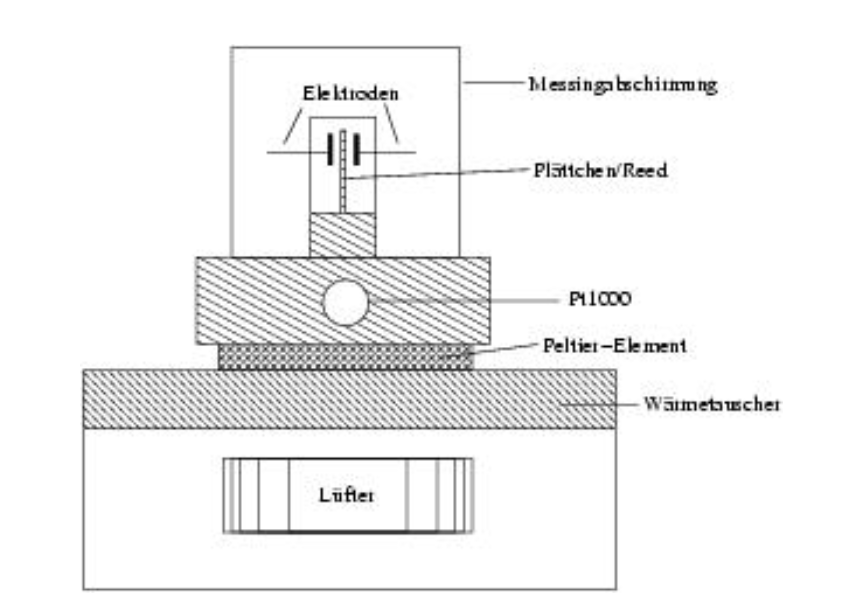
\includegraphics[width=\textwidth]{figures/VibrReedSchema.png}
        \caption*{(a) Schematischer Aufbau}
    \end{minipage}
    \hfill
    \begin{minipage}[t]{0.48\textwidth}
        \centering
        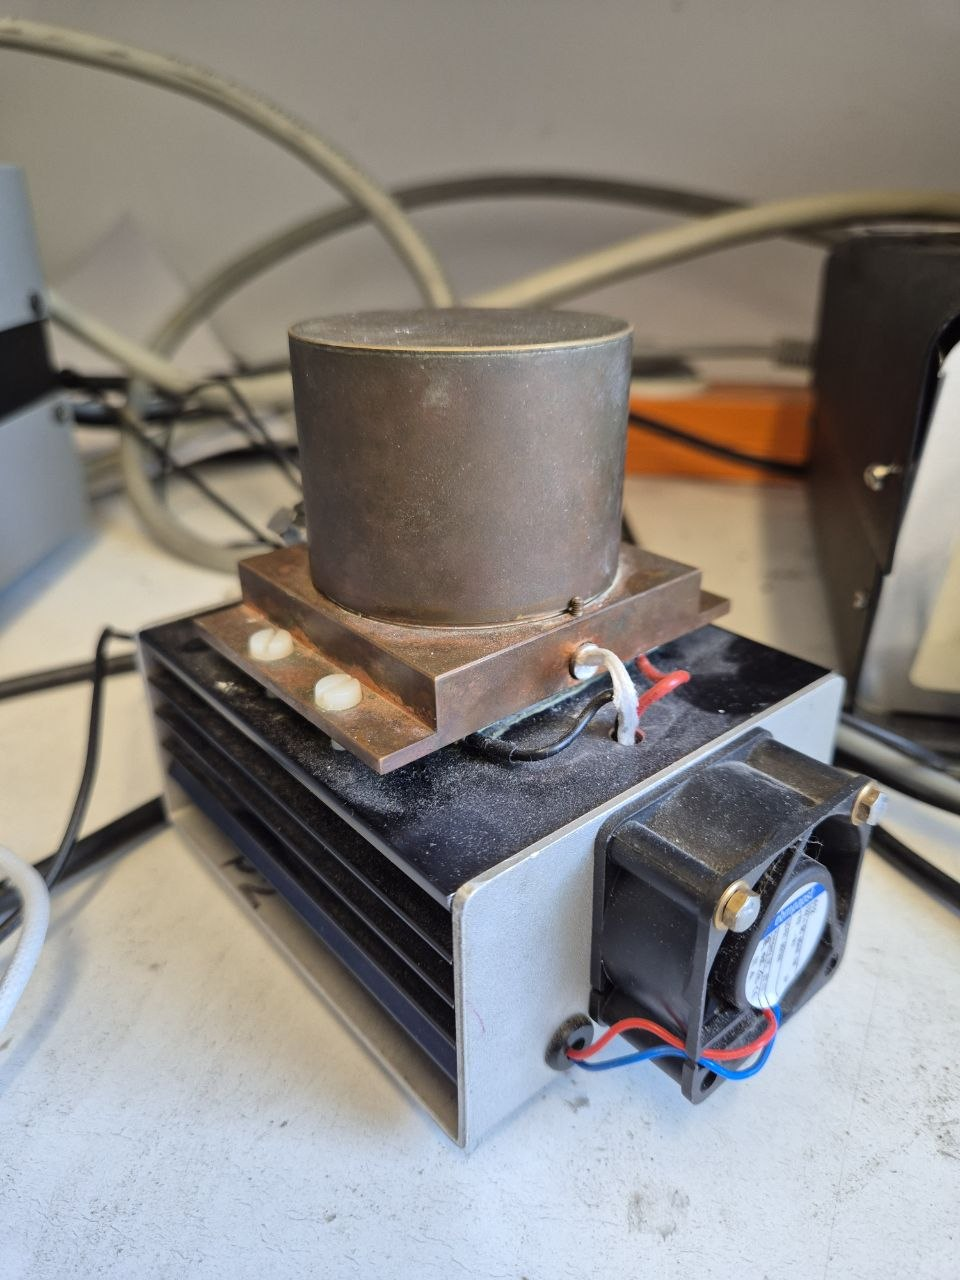
\includegraphics[width=\textwidth]{figures/Vibrator.jpeg}
        \caption*{(b) Tatsächliches Gerät}
    \end{minipage}

    \caption{Mechanischer und thermischer Aufbau des Vibrating-Reed-Experiments.}
    \label{fig:mechanischer_aufbau}
\end{figure}





\subsection{Elektronischer Aufbau}
Der Frequenzgenerator SRS DS345 liefert eine sinusförmige Anregungsspannung. Da die elektrostatische Kraft proportional zum Quadrat der angelegten Spannung ist, schwingt das Reed mit der doppelten Generatorfrequenz. Im Messprogramm wird daher die an den Generator übertragene Frequenz $\nu_G$ später mit dem Faktor zwei multipliziert und als mechanische Frequenz
\begin{equation}
    \nu=2\nu_G
\end{equation}
gespeichert.

Das Detektionssignal wird mit dem Zwei-Phasen-LoVe SRS SR530 aufgenommen, welcher zwei Signale konstanter Spannung ausgibt: 
\begin{equation}
    X=A\cos\varphi,
    \qquad
    Y=A\sin\varphi
\end{equation}
\(\phi\) ist die relative Phase zwischen Eingangsignal und Referenzsignal des LoVe. Über die Befehle \texttt{QX} und \texttt{QY} werden die beiden Komponenten \(X,Y\) ausgelesen.

Die Kommunikation mit allen Geräten erfolgt über einen Prologix-GPIB-USB-Controller: Jeder Befehl enthält die Adresse des adressierten Gerätes und die vom Skript vorgegebene Syntax, um ein Signal einzustellen und auszulesen. Am Beispiel des Frequenzgenerator mit Adresse 19:\\
\verb|gpib.write(19, "FREQ {:.3f}".format(freq))| mit \(\texttt{freq}=\nu_G\)\\
\verb|gpib.query(19, "FREQ?")|.

\section{Auswertung}
Die aufgenommnen Daten liegen in Form von \verb|.csv| Dateien vor und zeigen keine groben Auffälligkeiten oder fehlerhafte Speicherung. 

Alle im folgenden benutzten Formeln und Gleichungen, die das Modell der harmonischen Reed-Schwingung beschreiben, sind aus der Versuchsanleitung/Skript \autocite{Skript} übernommen und werden dementsprechend nicht einzeln mit Zitierbelegen ausgestattet. 

\subsection{Statistische Methode und Fitqualität}

Die Evaluierung der Fitmodelle erfolgt durch Minimierung der \(\chi_2\) Summe:
\begin{equation}
    \chi^2=\sum_{i=1}^{N}\left(\frac{y_i-f(x_i;\boldsymbol{a})}{\Delta y_i}\right)^2.
    \label{eq:chi2}
\end{equation}
Wobei \(\{y_i(x_i)\}_i^N\) die Familie der experimentellen Messwerte mit zugehörigem Fehler \(\Delta y_i\) bezeichnet und \(f(x_i;\boldsymbol{a})\) die durch das Fitmodell mit den Parametern \(\boldsymbol{a}=(a_1,\dots,a_p)\) bestimmten Werte sind. Die Fitparameter werden als unkorreliert angenommen, sodass sich die Unsicherheit jedes Fitparameters durch den Diagonaleintrag der Kovarianzmatrix bestimmen lässt: \(\Delta a_i=\sqrt{\operatorname{diag}_i(\texttt{pcov})}\). Mit $p$ Fitparametern beträgt die Zahl der Freiheitsgrade
\begin{equation}
    n_{\mathrm{df}}=N-p.
\end{equation}
Zur Beurteilung werden $\chi^2$, $\mathrm{red}\;\chi^2= \chi^2/n_{\mathrm{df}}$, die zugehörige Fitwahrscheinlichkeit (mithilfe der python libary \libary{scipy.stats.chi2} und Funktion $\verb|chi2.cdf|$ berechnet)\autocite[128]{Skript_2.1} und die Residuen (engl.\ \emph{residuals}) betrachtet. Ein stark erhöhtes reduziertes $\chi^2$ kann auf unterschätzte Unsicherheiten, systematische Effekte oder ein unzureichendes Modell hinweisen. Ein stark erniedrigter Wert kann auf überschätzte beziehungsweise korrelierte Unsicherheiten hindeuten.

Die normierten Residuen werden folgend berechnet:
\begin{equation}
    \mathrm{residuals}=\frac{y_i-f(x_i)}{\Delta y_i}.
    \label{eq:residuen}
\end{equation}


\subsection{Versuchsabschnitt A: Resonanzkurven der Moden 0,1,2}
\subsubsection{Messprinzip}
Folgendes gilt für alle drei zu untersuchenden Resonanzmoden \(n\in\{0,1,2\}\): In einem durch Testscans festgelegten Frequenzintervall \(\nu_n-d<\nu_n<\nu_n+d\) um die Resonanzfrequenzen \(\nu_n\) werden mit einer durch \(d\) und \(N\) einstellbaren Stepsize \(\Delta \nu=\frac{2d}{N}\) \(N\) Frequenz-Datenpunkt-Tupel der Form \((\nu;X,Y)\) erhoben, wobei von \(X,Y\) zur Bildung eines stochastischen Fehlers (Fehler des Mittelwerts) \(M=20\) Messungen erhoben werden. 
\begin{align}
    \bar{X}&=\frac{1}{M}\sum_{i=1}^{M}X_i &
    \Delta X&=\frac{1}{\sqrt{M}}\sqrt{\frac{1}{M-1}\sum_{i=1}^{M}(X_i-\bar{X})^2}\\
    \intertext{Mithilfe von}
    A&=\sqrt{\bar X^2+\bar Y^2} & \varphi&=\operatorname{atan2}(\bar Y,\bar X).
\end{align}
wird die Amplitude und die Phase berechnet, deren Unsicherheiten werden dabei automatisch mit dem  Paket \texttt{uncertainties} aus den Fehlern von $\bar X$ und $\bar Y$ fortgepflanzt. Die Verwendung von atan2 stellt sicher, dass bei der Phasenberechnung der richtige Quadrant
berücksichtigt wird. Die Datenpunkttupel \((\nu;X,\Delta X,Y,\Delta Y,A,\Delta A,\varphi,\Delta \varphi)\) werden anschließend in einer \verb|.csv| Datei durch eine \verb|DataWriter| Klasse gespeichert. Der gesamte Code findet sich in der im selben Heibox Ordner liegenden Datei \textcolor{blue}{\texttt{\detokenize{Final_PC2_Code.ipynb}}}.

\subsubsection{Ziel und vollständiger Arbeitsablauf}
Zunächst werden die drei Resonanzen mit kurzen, groben Scans (\(M=150\)) lokalisiert. Danach wird für jede Mode ein eigener endgültiger Messbereich der Breite \(d\) um \(\nu_n\) gewählt. Eine \verb|Measurement| Klasse wird initialsiert, die durch die Hauptfunktion \verb|Measurement.measure_curve| eine Resonanzkurve mit \(N\) Datenpunkten aufnimmt. Die Informationen der \verb|.csv| Datei werden durch Plotten der Resonanzkurven \(A(\nu)\) sowie \(X(\nu),Y(\nu)\) und der Phase \(\varphi(\nu)\) auswertet. Als zusätzliche Funktionalität werden nach jedem abgeschlossen Arbeitsschritt (Aufnehmen der ersten Resonanzkurve,usw.\ ) sowohl die benötigte Zeit gespeichert, als auch zur ansatzweisen Remote-Beaufsichtigung eine Email an die Experimentatoren gesendet.\footnote{Dies wurde mit der Funktion EmailMessage aus dem Python-Paket email.message realisiert und erforderte lediglich das Erstellen eines App-Passworts für den verwendeten Google-Account. Es handelt sich dabei um eine ausgesprochen nützliche Funktioni, die die Experimentatoren davor noch nicht kannten und in Zukunft wohl noch oft verwenden werden.}


\subsubsection{Darstellung der Messdaten}
Es wurden zwei Versuchsaufbauten (bezeichnet mit PC1 und PC2) untersucht, um vergleichbare Daten zu zwei unterschiedlichen Reeds zu erheben.

Allgemein wird erwartet, dass sich die Amplitudendaten im zentralen Resonanzbereich durch das Fitmodell einer Lorentzform beschreiben lassen sollten:

\begin{equation}
    f(\omega; f_0, \omega_{0,n}, \gamma) = \frac{f_0}{\sqrt{(\omega_{0,n}^2 - \omega^2)^2 + (\gamma \omega)^2}}+y_0
    \label{eq:fit_amplitude}
\end{equation}
Die freien Parameter sind:
\begin{itemize}
    \item Konstante \(f_0\)
    \item \(\omega_{0,n}\) die Resonanzkreisfrequenz
    \item \(\gamma\;[\unit{\rad\per\s}]\) die Dämpfungskonstante
    \item \(y_0\) Untergrund
\end{itemize}
Nutzt man die Näherung kleiner Dämpfung und \(y_0\approx 0\), folgt aus: 
\begin{equation}
    \omega_R=\sqrt{\omega_0^2-\frac{\gamma^2}{2}}\approx\omega_0\implies A_{\mathrm{max}}=f(\omega_0=\omega_R)\implies f_0=A_R\,\gamma\,\omega_0
\end{equation}
Dann wäre dieser freie Paremter direkt als Amplitude \(A_R\)  an der Resonanzfrequenz interpretierbar. Die Näherung kleiner Dämpfung trifft in den untersuchten Systemen zwar zu, um jedoch so nahe wie möglich an der Aufgabenstellung des Skripts zu bleiben, wurde mit dem Parameter \(f_0\) gearbeitet. Um numerische Probleme beim Fitten von kleinen Zahlen präventiv zu vermeiden, werden die Amplitudendaten vorher auf 1 normiert, also optimalerweise beträgt \(A_R\approx1\).

\newpage

\subsubsection{Fitresultate}
\paragraph{PC1:}
\begin{figure}[htbp]
\centering
    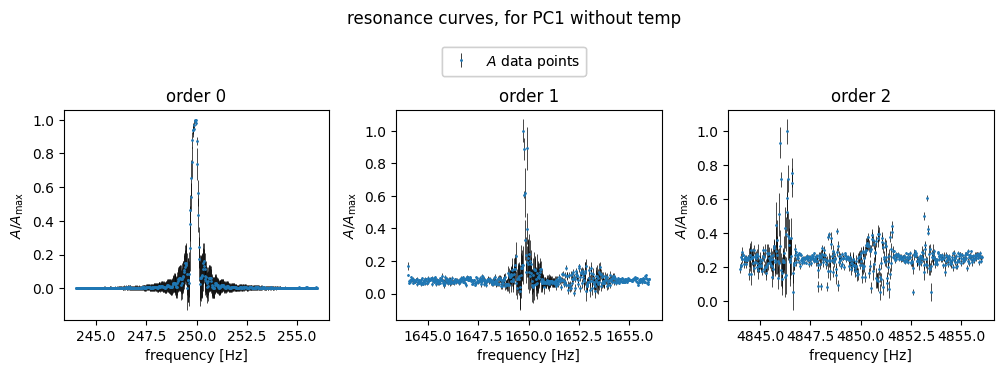
\includegraphics[width=\textwidth]{figures/PC1/Plot__ResFreq.png}
    \caption{PC1: Messdatenüberblick der Moden 0,1,2}
    \label{fig:PC1_n012}
\end{figure}
\FloatBarrier

Die Messung für \(\nu_0\) wurde über einen Frequenzbereich von \(\qtyrange{244}{256}{\hertz}\) mit 500 Steps, also einer Schrittweite von \(\Delta \nu=\qty{0.024}{\hertz}\) aufgenommen. Die Breite der Resonanzkurve beträgt nur wenige Hertz, weswegen der dargestellte Frequenzbereich und Fit nur 166 Datenpunkte inkludiert.

\begin{figure}[htbp]
\begin{subfigure}[b]{0.48\textwidth}    
    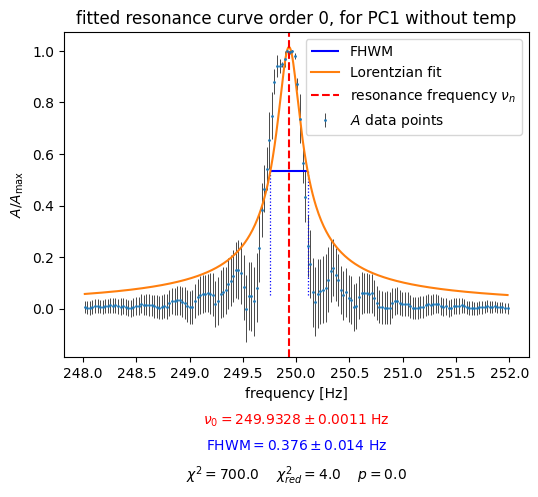
\includegraphics[width=\linewidth]{figures/PC1/Fit__ResFreq0.png}
    \caption{Resonanzkurve 0}
    \label{fig:PC1_n0}
\end{subfigure}
\hfill
\begin{subfigure}[b]{0.48\textwidth}
    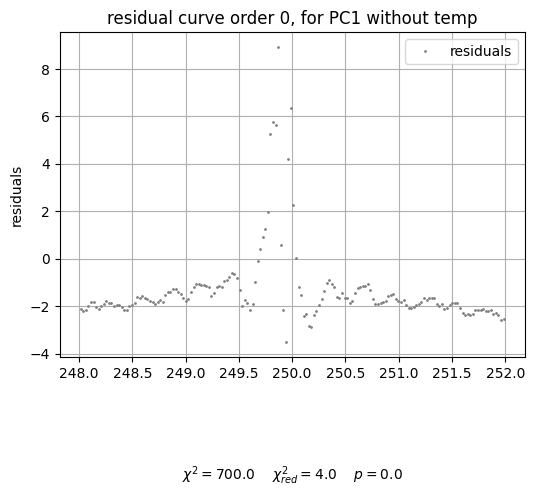
\includegraphics[width=\linewidth]{figures/PC1/Plot_residuals__ResFreq0}
    \caption{Residuals}
\end{subfigure}
    \caption{PC1: Resonanzkurve 0 und residuals}
    \label{fig:nu_0_residuals_PC1}
\end{figure}
\FloatBarrier

Damit ist \(\chi_2=740\gg \mathrm{dof}=162\), das Fitmodell ist zur Beschreibung der Messdaten nicht geeignet.
Die Residuals \(\frac{A(\nu_i)-f(nu_i)}{\Delta A(\nu_i)}\) zeigen, wie am Fit schon augenfällig wird, eine systematische Überhöhung des Fits. Eine Erklärung liefert die Verteilung der beobachteten Datenpunkte: Eine nenneswerte Resonanz (Amplitudenverstärkung, die sich relevant vom Untergrund abhebt), beschränkt sich auf wenige Hertz, zeigt also nur für wenige Datenpunkte ein Ansteigen der Amplitude. Die charakteristische Breite - also das Beobachten einer geweiteten Kurve, ist nicht erkennbar.

Die Güte der Resonanzkurve lässt sich sowohl nur mithilfe der Fit-Parameter als auch in Kombination mit der grafisch bestimmten Halbwertsbreite bestimmen:


\begin{equation}
    \begin{aligned}
        Q_n &= \frac{\omega_{0,n}}{\gamma},\\
        \Delta Q_n &= Q_n\sqrt{
            \left(\frac{\Delta \omega_{0,n}}{\omega_{0,n}}\right)^2
            +\left(\frac{\Delta \gamma}{\gamma}\right)^2
        },\\
        Q_0 &= \num{1150(40)}
    \end{aligned}
\end{equation}

\begin{equation}
    \begin{aligned}
        Q_{\text{graf}} &= \sqrt{3}\frac{\nu_R}{\mathrm{FWHM}},\\
        \Delta Q_{\text{graf}} &= Q_{\text{graf}}\sqrt{
            \left(\frac{\Delta \nu_R}{\nu_R}\right)^2
            +\left(\frac{\Delta \mathrm{FWHM}}{\mathrm{FWHM}}\right)^2
        },\\
        Q_{\text{graf}} &= \num{1240(150)}
    \end{aligned}
\end{equation}

Der Fehler wurde auf \(\Delta \mathrm{FHWM}=\sqrt{2}\;\qty{0.024}{\hertz}\), also in der Größenordnung der Stepsize gesetzt. \textit{Anmerkung/Frage: Wie bestimmt man korrekt den Fehler eine grafischen FHWM?}
Ein Gütefaktor in dieser Größenordnung (angesichts der nicht interpretierbaren Ergebnisse der anderen  Resonanzmoden) lässt scheinbar auf eine sehr hohe Frequenzstabilität des Reeds im Betriebsbereich um die Resonanzfrequenz schließen. Der Unterschied zwischen Methoden der Gütenbestimmung beträgt \(S[\sigma]=\num{0.6}\sigma\).
Die Aussagekraft des Ergebnisses \(Q_1=\num{40000(7000)}
\) aus \zcref{fig:nu1_PC1} ist angesichts der geringen Anzahl an verfügbaren Datenpunkten fragwürdig. Somit wird ein Vergleich von \(Q_{0,1,2}\) für PC1 ausgelassen. 

Im Gegensatz zur Erwartung, dass \(\varphi\approx\{0|\nu<\nu_n;\frac{\pi}{2}|\nu\approx\nu_n;\pi|\nu>\nu_n\}\) und damit einem entsprechenden Verhalten von \(X=A\cos\varphi,Y=A\sin\varphi\) zeigen sich für die Phase und \(X,Y\) folgende nicht weiter analysierbare Verhaltensweisen:

\begin{figure}[htbp]
\begin{subfigure}[b]{0.48\textwidth}    
    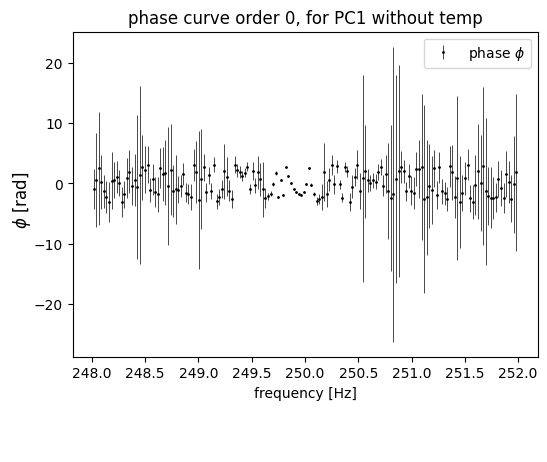
\includegraphics[width=\linewidth]{figures/PC1/Plot_phase__ResFreq0.png}
    \caption{Phase \(\varphi\)}
\end{subfigure}
\hfill
\begin{subfigure}[b]{0.48\textwidth}
    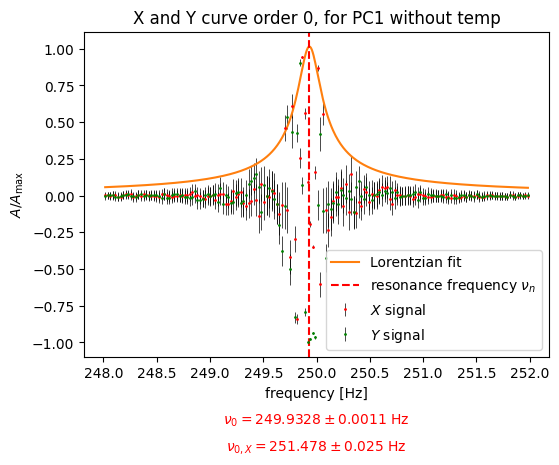
\includegraphics[width=\linewidth]{figures/PC1/Fit_xy__ResFreq0.png}
    \caption{\(X,Y\)}
\end{subfigure}
    \caption{PC1: \(X,Y,\varphi\) gegen Frequenz aufgetragen - nicht interpretierbare Resultate}
    \label{fig:XY_Phase_PC1}
\end{figure}
\FloatBarrier

Es ist augenfällig, dass kein wie im Skript erwarteter Nulldurchgang von \(X=A\cos\varphi\) als Vergleichswert für die Resonanzfrequenz dienen kann. 
Die PC1-Ergebnisse entsprechen in vielerlei Hinsicht nicht den theoretischen Erwartungen, ein Vergleich zwischen \(\chi_2\) und der Anzahl an Freiheitsgraden dof ergibt: \(\chi_2\gg \mathrm{dof})\), was auf systematische Fehler hindeutet bzw. auf die wahrscheinlichere Option: Der vorliegende Experimentieraufbau PC1 lässt sich mit dem theoretischen Modell nicht beschreiben. Diese Schlussfolgerung wird durch die Resonanzkurven der Moden \(n=1,2\) unterstrichen:

\begin{figure}[htbp]
\begin{subfigure}[b]{0.48\textwidth}    
    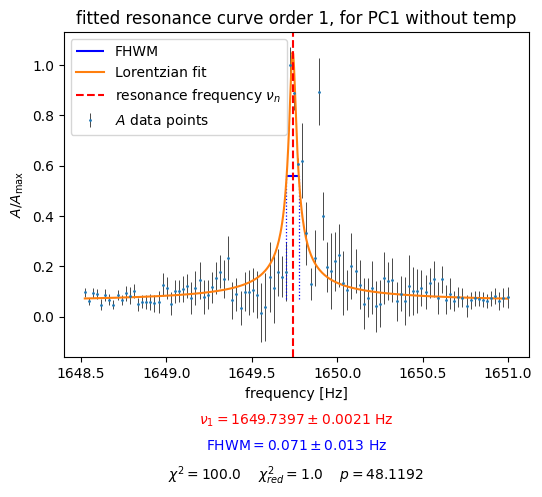
\includegraphics[width=\linewidth]{figures/PC1/Fit__ResFreq1.png}
    \caption{Erste Schwingungsmode}
    \label{fig:nu1_PC1}
\end{subfigure}
\hfill
\begin{subfigure}[b]{0.48\textwidth}
    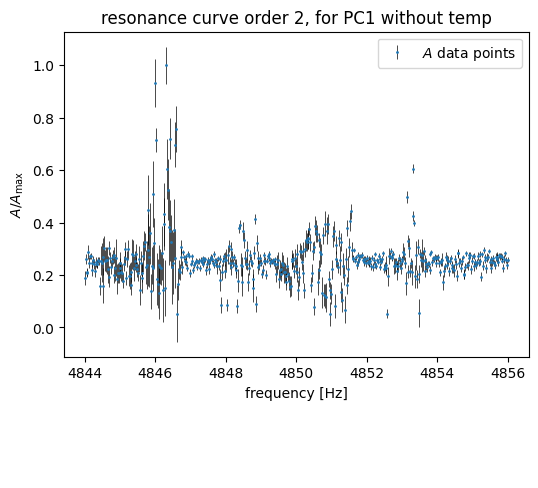
\includegraphics[width=\linewidth]{figures/PC1/Plot__ResFreq2.png}
    \caption{Zweite Schwingungsmode}
\end{subfigure}
    \caption{PC1: Resonanzkurven/Messdaten von \(\nu_1,\nu_2\)}
    \label{fig:nu12_PC1}
\end{figure}
\FloatBarrier

An die Messdaten des ersten Modenbereichs lässt sich zwar eine Resonanzkurve fitten, die effektiv jedoch nur aus wenigen Datenpunkten besteht. Das Verhältnis zur nullten Mode beträgt \(\frac{\nu_1}{\nu_0}=\num{6.60073(0.00004)}\), die Abweichung zum Literaturwert beträgt somit \(S[\sigma]=\num{700}\sigma\). Die Größenordnung stimmt jedoch sehr gut überein, das lässt vermuten/hoffen, dass die beobachteten Kurven in der Tat Resonanzkurven sind. Die Datenpunkte des Messbereichs um die theoretisch berechnete Resonanz \(\nu_2\) (in den Testdaten zur Auffindung der Resonanz wurde durch niedrigere Stepsize das Datenpunktcluster um \(\qty{4845}{\hertz}\) als Resonanzbereich abgeschätzt) lassen keine weitere Analyse zu, das Fitten einer Resonanzkurve ist nicht möglich. 

\paragraph{PC2}
Im Gegensatz zu PC1 zeigt sich eine breite Resonanzkurve über mehrere hundert Hertz. Der Fitbereich wird nicht eingeschränkt, da kein nennenswerter \enquote{Untergrund-Tail} aufgenommen wurde. Dafür PC2 wurden allerdings Messpunkte ausgeschlossen, bei denen der LoVe in Sättigung geriet (bei der Nullten Mode): Die beiden gemessenen Quadraturkomponenten $X=A\cos\varphi$ und $Y=A\sin\varphi$ erreichen bei unterschiedlichen Frequenzen jeweils einen konstanten Maximalwert. Da die Amplitude aus $A=\sqrt{X^2+Y^2}$ berechnet wird, führt diese Begrenzung der einzelnen Komponenten zu einer künstlichen Verformung der Resonanzkurve (einem scheinbaren zweiten Maximum). Zur Identifikation solcher Bereiche wurden im Auswertungscode zusammenhängende Plateaus von mindestens fünf Messpunkten nahe dem jeweiligen Maximalwert von $X$ oder $Y$ gesucht. Die betroffenen Messpunkte wurden vom Fit ausgeschlossen, in den Diagrammen jedoch weiterhin grau dargestellt. Somit wurden ausschließlich die als gesättigt identifizierten Werte verworfen; andere auffällige Messpunkte blieben zunächst erhalten.


\begin{figure}[htbp]
\centering
    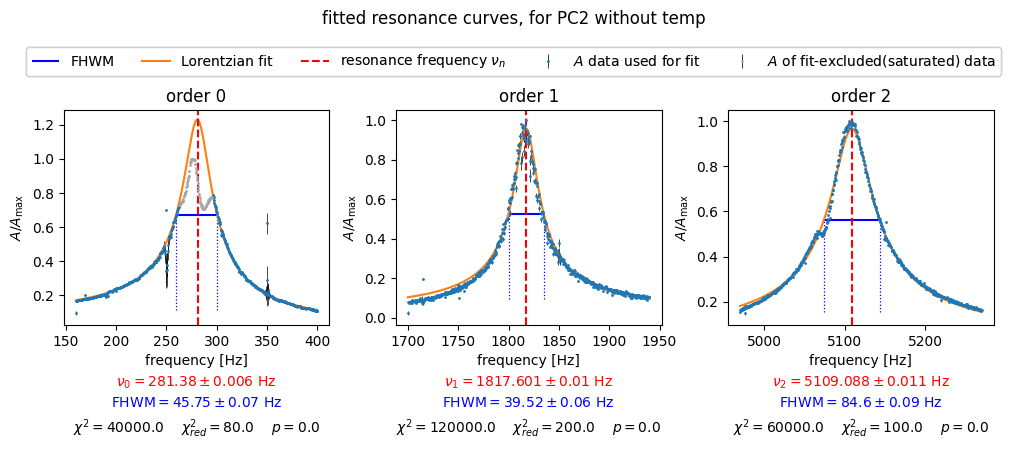
\includegraphics[width=\textwidth]{figures/PC2/Fit__final_ResFreq.png}
    \caption{PC2: Resonanzkurven der Moden 0,1,2}
    \label{fig:PC2_n012}
\end{figure}
\FloatBarrier
Ein Einschränken des Frequenzbereiches lieferte keine signifikant besseren Fitergebnisse.
Die zu bestimmenden Resultate werden, da nun alle drei Kurven analysierbare Ergebnisse zulassen, in der folgender Tabelle dargestellt:

\begin{table}[htbp]
  \centering
    \caption{PC2: Fitresultate der drei Resonanzkurven.}
  \begin{tabularx}{\textwidth}{lZZZZx}
    \toprule
    Mode & \nu_R\;[\unit{\hertz}] & \gamma\;[\unit{\rad\per\s}] & Q & Q_{\text{graf}} & S_{QQ}[\sigma]\\
    \midrule
    0 & \num{281.380(0.006)} & \num{166.33(0.22)} & \num{10.629(0.015)} & \num{11.89(0.18)} & \num{7}\\
    1 &  \num{1817.601(0.010)} & \num{143.37(0.18)} & \num{79.66(0.11)} & \num{89.7(1.6)} & \num{7}\\
    2 & \num{5108.971(0.012)} & \num{306.9(0.3)} & \num{104.60(0.11)} & \num{127.0(1.5)} & \num{15}\\
    \bottomrule
  \end{tabularx}
\label{table:PC2_Fitresults}  
\end{table}
Erste Bemerkung sei noch: Numerisches Berechnen zeigt: \(\omega_R=\sqrt{\omega_0^2-\gamma^2/2}=\omega_0\). Zudem ist der Fitparameter des Untergrunds \(y_0\approx\num{0}\) für alle Moden. Die Signal-zu-Rausch-Verhältnisse, die durch den nächsten Messdatenpunkt \(\nu_i\) neben der gefitteten Resonanzfrequenz \(\nu_R\) definiert sind:
\begin{equation}
    V={A_{\max}}/{\Delta A_{\max}
    \qquad \text{ mit } A_{\max}(\nu_{\max})=
    \set{A(\nu)}{\min_i \nu_R-\nu_i} 
    },
\end{equation}
betragen \(V_{0,1,2}=\numlist{900;500;240}\), für eine Einschätzung dieser Verhältnisse fehlt die Expertise.
Die Güte steigt bei höherer Modenzahl, die absolute Abweichung zwischen grafisch ermittelter Güte und berechneter Güte steigt ebenso. Dieser Effekt ist verwunderlich, wird doch die grafische Güte aus der Fitkurve ermittelt und mit dem Fitparameter \(\omega_R=\omega_0\) verrechnet.

Die Frequenzverhältnisse sind:
\begin{table}[htbp]
\centering
\caption{PC2: Vergleich der Frequenzverhätlnisse mit Literaturwert}
\begin{tabularx}{\textwidth}{xZxZZx}
    \toprule
         n & V=\frac{\nu_{n}}{\nu_0} & V_{\text{Lit}} & \text{abs.Abw.} & \text{proz.Abw.}[\unit{\percent}] & S[\sigma] \\\midrule
        1 & \num{6.47367(0.00017)} & 6.267 & \num{0.15333(0.00017)} & \num{2.369(0.003)} & 1000.0 \\
       2 & \num{18.1971(0.0005)} & 17.548 & \num{0.6491(0.0005)} & \num{3.567(0.003)} & 1300.0 \\
\bottomrule
\end{tabularx}
\label{table:Vergleich_V_i} 
\end{table}

Die absolute und relative Abweichung sehr gut, die Signifikanz wird durch die winzigen Fehler der Verhältnisse verzerrt. \textit{Frage:} Warum sind die Kovarianzfehler von \(\nu_n\) so gering? Liegt das an den geringen Fehlern \(\Delta A\)? Denn folglich ist auch \(\Delta V\) sehr gering.

Auch die Phasenbilder zeigen das gewünschte, oben beschriebene Verhalten: 
\begin{figure}[htbp]
\centering
    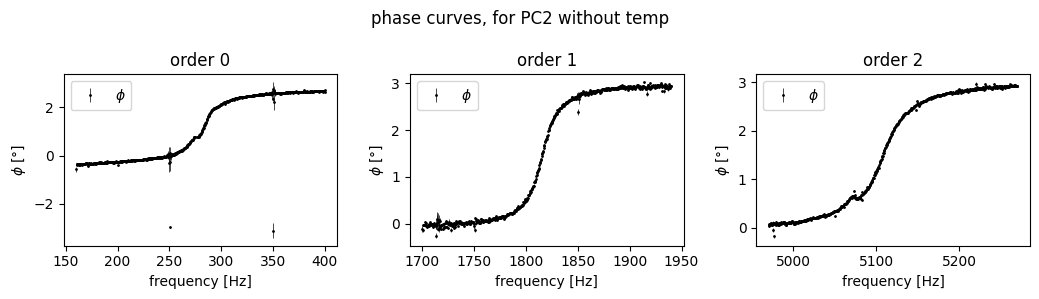
\includegraphics[width=\textwidth]{figures/PC2/Plot_phase__final_ResFreq.png}
    \caption{PC2: Phasenkurven der Moden 0,1,2}
    \label{fig:PC2_n012_phase}
\end{figure}
\FloatBarrier

 Damit lassen sich wie in \autocite[28]{Skript} auch die erwarteten \(X=A\cos\varphi,\,Y=A\sin\varphi\) beobachten:

\begin{figure}[htbp]
\centering
    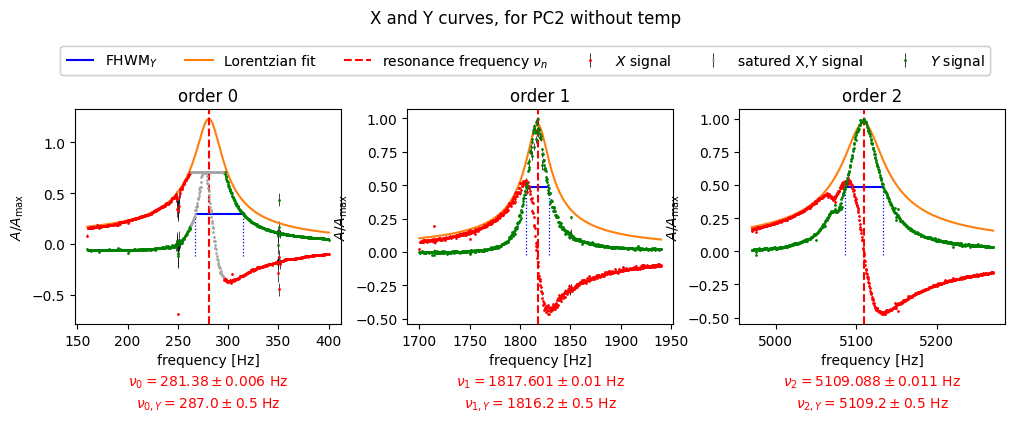
\includegraphics[width=\textwidth]{figures/PC2/Fit_xy__final_ResFreq.png}
    \caption{PC2: X,Y Kurven der Moden 0,1,2}
    \label{fig:PC2_n012_XY}
\end{figure}
\FloatBarrier
Die Halbwertsbreite \(\mathrm{FHWM}_Y\) des \(Y\)-Signals der ersten Mode muss verworfen werden, da der LoVe offensichtlicherweise in Wolke 7 (respektive Sättigung) ist. Die Güte des Reeds kann für \(\nu_{1,2}\) auch mit dem \(Y\)-Signal berechnet werden: \(Q_{Y}={f_{R}}/{\mathrm{FHWM_{Y}}}\)\autocite[27]{Skript}:

\begin{table}[htbp]
\centering
    \caption{PC2: Vergleich der Gütenbestimmung über \(X,Y\) mit berechneter Güte}
\begin{tabularx}{\textwidth}{xZZZZx}
    \toprule
         n & Q & Q_{Y,\text{ graf}} & \text{abs. Abw.} & \text{proz. Abw.}[\unit{\percent}] & S[\sigma] \\\midrule
       0 & \num{10.629(0.015)} & - & - & - & - \\
       1 & \num{79.66(0.11)} & \num{79.7(1.8)} & \num{0.0(1.9)} & \num{0.1(2.3)} & \num{0.023} \\
       2 & \num{104.60(0.11)} & \num{107.3(1.2)} & \num{2.7(1.3)} & \num{2.6(1.2)} & \num{2.3} \\
\bottomrule
\end{tabularx}
\label{table:PC2_Fitresults_for_Q} 
\end{table}
Für diese Signifikanzen hat sich doch die ganze Arbeit gelohnt.

Zudem wurde wie im Skript gefordert, aus dem Nulldurchgang von \(X=A\cos\varphi\) die zugehörige Frequenz ermittelt:
\begin{table}[htbp]
\centering
\caption{PC2: Vergleich von $\nu_{R,n}$ und $\nu_{R,n; \text{Null}}$}
\begin{tabularx}{\textwidth}{xZZZZx}
    \toprule
        n & \nu_{R}\,[\unit{\hertz}] & \nu_{R; \text{Null}}\,[\unit{\hertz}] & \text{abs.\ Abw.}\,[\unit{\hertz}] & \text{proz.\ Abw.}\,[\unit{\percent}] & S[\sigma] \\\midrule
      0 & \num{280.757(0.007)} & \num{287.0(0.4)} & \num{6.3(0.5)} & \num{2.23(0.15)} & \num{16} \\
       1 & \num{1817.529(0.011)} & \num{1816.2(0.4)} & \num{1.3(0.5)} & \num{0.073(0.023)} & \num{4} \\
       2 & \num{5108.971(0.012)} & \num{5109.2(0.5)} & \num{0.3(0.6)} & \num{0.005(0.010)} & \num{0.6} \\
\bottomrule
\end{tabularx}
\label{table:PC2_Vergleich_nu_{R,n,0}} 
\end{table}
\FloatBarrier

An den niedrigen absoluten Abweichungen ist eine gute Übereinstimmung erkennbar. Als Fehler für die Nulldurchgangsfrequenz wurde wie oben die zugrundeliegende Stepsize der Messung verwendet. 

Final seien auch hier der Vollständigkeit halber die residuals geplottet:
\begin{figure}[htbp]
\centering
    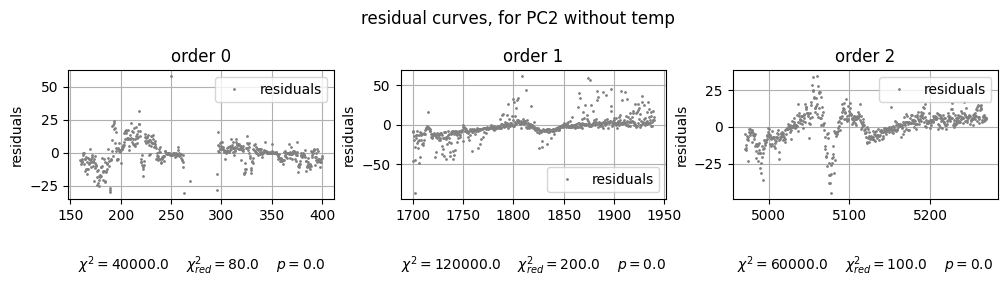
\includegraphics[width=\textwidth]{figures/PC2/Plot_residuals__final_ResFreq.png}
    \caption{PC2: residuals der Moden 0,1,2}
    \label{fig:PC2_n012_residuals}
\end{figure}
\FloatBarrier
Wiederum stellt sich die Frage mangels Expertise: Ist hier ein Muster erkennbar, welches darauf schließen lässt, dass das Fitmodell angepasst werden müsste, wie in \autocite[27]{Skript} beschrieben? Es ist nicht davon auszugehen, da die in \zcref{fig:PC2_n012} abgebildeten Messdaten einen klaren Lorentzfunktionen-Verlauf zeigen, also resonanzcharakterisch sind.

\subsection{Versuchsabschnitt B: Temperaturabhängigkeit}

Im zweiten Teil des Versuchs beschränken wir uns nun auf die nullte Mode des Reeds und untersuchen die Änderungen der Resonanzkurve bei unterschiedlichen Temperaturen. Hierzu wird das Reed mit dem eingebauten Peltierelement (siehe \zcref{fig:mechanischer_aufbau}) zu Temperaturen zwischen etwa $36^\circ$ C und $60^\circ$ C aufgeheizt. Dass die niedrigsten Temperaturen so hoch sind liegt daran, dass das Experiment im August 2026 durchgeführt wurde und die Temperaturen im Labor selbst bereits bei etwa $37^\circ$C lagen. 

Eine Schwierigkeit bei der Einstellung des Peltierelements ist, dass dieses lediglich durch festlegen der Spannung (Werte zwischen 0 V und 2 V erlaubt) angesprochen werden kann und keine Möglichkeit zur Umrechnung von Spannung und Temperatur zur Verfügung gestellt wurde. Den Zusammenhang selbst experimentell festzustellen hätte lange gedauert, da für jeden Aufnahmepunkt einige Zeit gewartet werden müsste, bis sich die zu einem bestimmten Spannungswert gehörende Temperatur eingestellt hat. Überdies ist davon auszugehen, dass die Raumtemperatur (die sich über Nacht stark ändern kann) beeinfluss, welche Spannung am Peltierelement zu welcher Temperatur im Reed führt. Aus diesem Grund wurde ein dynamischer Regelungsalgorithmus auf die folgende Art einprogrammiert.


\subsubsection{Temperaturregelung}
 Der implementierte Algorithmus lässt sich als inkrementeller Dreipunktregler mit adaptiver Schrittweite beschreiben. Hierbei wird zunächst die aktuelle Temperatur $T_k$ als Mittelwert aus fünf Messungen im Abstand von jeweils einer Sekunde bestimmt und mit der Solltemperatur $T_\mathrm{soll}$ verglichen. Abhängig von der Regelabweichung wird die Spannung $U_k$ am Peltierelement erhöht, verringert oder unverändert gelassen. Die Aktualisierung erfolgt nach
\begin{equation} \label{eq:U-update}
    U_{k+1} = \mathrm{clip}(U_k + \eta_k d_k,\;0,\;1{,}95\,\mathrm{V}),
    \qquad
    d_k =
    \begin{cases}
        +1 & T_k < T_\mathrm{soll}-\delta T,\\
        0 & |T_k-T_\mathrm{soll}|\leq\delta T,\\
        -1 & T_k > T_\mathrm{soll}+\delta T,
    \end{cases}
\end{equation}
mit der Toleranz $\delta T=1{,}5\,^\circ\mathrm{C}$ und der dynamischen Schrittweite $\eta_k$. Als Startwert $U_0$ wird am Anfang der Messung $U_0=0{,}1$V gesetzt. Die clip-Funktion sorgt dafür, dass 0 V und 2 V dabei zu keinem Zeitpunkt über- bzw. unterschritten werden können. Dass eine höhere Spannung zu einer höheren Temperatur führt wird vorausgesetzt, prinzipiell wird die Spannung also schlicht verringert, falls die aktuelle Temperatur zu hoch, bzw erhöht falls sie zu niedrig ist. Diese Änderung (Schrittweite $\eta_k$) wurde dabei nicht proportional zur Abweichung (P-Regler) gewählt, da von einem verspäteten Feedback bei der Temperatureinstellung auszugehen ist und die echte Abweichung daher nicht immer instantan bekannt ist. 

Stattdessen wird die Schrittweite $\eta_k$ erhöht und verringert, je nachdem \emph{wie oft} bereits erhöht werden musste, d.h. die Schrittweite wird größer, wenn bei vielen aufeinander folgenden Updates die aktuelle Temperatur in dieselbe Richtung von der Solltemperatur abweicht. So soll die Einstellung der Solltemperatur beschleunigt und gleichzeitig ein Überschwingen reduziert werden. Konkret wird $\eta$ gemäß

\begin{equation} \label{eq:eta-update}
    \eta_{k} = \mathrm{clip}(\alpha \cdot\eta_{k-1},\;0.01\,\mathrm{V},\; 0.5\, \mathrm{V})
    \qquad
    \alpha =
    \begin{cases}
        1 & d_{k-1} = 0,\\
        0.5 & d_{k-1} d_{k-2} =-1,\\
        \gamma & d_{k-1} d_{k-2} =1,
    \end{cases}
\end{equation}

verändert, wobei $d_k$ wieder das in \zcref{eq:U-update} definierte Vorzeichen der Abweichung (außerhalb des Toleranzbereichs) ist. Als Startparameter werden überdies $\eta_1=0{,}1$ und $d_{0}=d_{-1}=0$ gesetzt. Der Wert $\gamma$ wurde für unterschiedliche Messungen variiert, er betrug am Anfang $\gamma=1{,}1$ und später $\gamma=1{,}05$, um das Verhalten der Regelung zu verbessern. Wie oben sorgt die Clip-Funktion dafür, dass die Änderungsrate nie zu groß oder zu klein werden kann; die Produkte aus $d_{k-1}$ und $d_{k-2}$ prüfen, ob sich die \emph{Richtung} der Abweichung im vorherigen Schritt verändert hat.  Ein einzelnes Update (Anwendung von \zcref{eq:U-update,eq:eta-update}) wird, solange die Temperatur nicht im Sollbereich liegt, alle sechs Sekunden durchgeführt (die Zeit, die die Durchschnittsbildung über fünf Werte braucht). Bei Erreichen der Solltemperatur wird überdies sicherheitshalber weitere 5 Sekunden gewartet, ob diese auch im gewünschten Bereich bleibt. Ein Temperaturcheck (mit eventueller Regelung) wird vor der Aufzeichnung jedesx einzelnen Messpunkts durchgeführt. Um zu Verhindern, dass die Temperaturregelung unendlich lang ohne Ergebnis läuft, wurde außerdem festgelegt, dass die Regelung nach 100 Versuchen pro Messpunkt abgebrochen und Notfalls ein Messpunkt mit falscher Temperatur aufgezeichnet wird. 

Insgesamt ist dieser Regelungsalgorithmus das Ergebnis einer Improvisation am Ende eines langen Versuchstages, an dem die Temperaturmessungen schnell gestartet werden sollten. Wir erheben nicht den Anspruch, hiermit eine besonders schnelle oder intelligente Regelungslogik implementiert zu haben - Ziel war schlicht ohne lange Tests eine automatische Einstellung der Temperatur über Nacht zu ermöglichen. 


\subsubsection{Qualitative Unterscheidung der Resultate beider PCs}
Für die Aufnahme der temperaturgeregelten Messungen wurde die Mode \(n=0\) verwendet. \footnote{Bei PC2 wurde erst im Nachhinein klar, dass bei der ersten Mode \(n=1\) kein Sättigunsverhalten auftritt und so bessere Resultate möglich geworden wären.} In \zcref{fig:Qual_T_behave} sind die Messungen bei allen Temperaturen auf PC1 (links) und PC2 (rechts) aufgetragen; insgesamt zeigen sich scheinbar größere Verschiebungen bei PC1 im Gegensatz zu scheinbar eher schwacher Temperaturabhängigkeit bei PC2. Zu beachten ist jedoch der unterschiedlich große untersuchte Bereich auf der x-Achse. Dieses Verhalten wird in den folgenden Abschnitten quantitativ untersucht. 

\begin{figure}[htbp]
\begin{subfigure}[b]{0.48\textwidth}    
    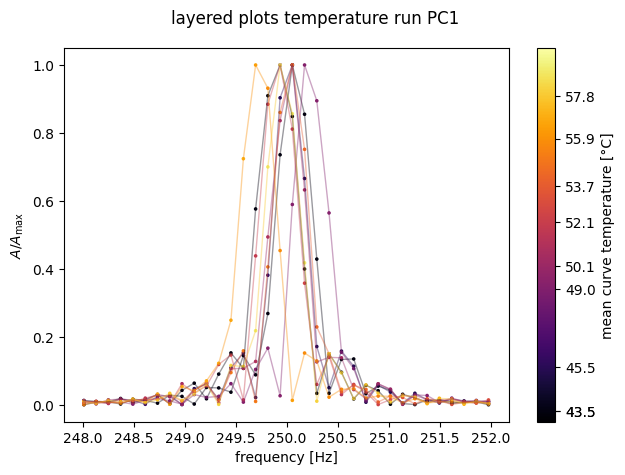
\includegraphics[width=\linewidth]{figures/PC1/Plot_temp_resonance_curves_TempFreq.png}
    \caption*{PC1: schmale Resonanzenkurven, chaotische Temperaturabhängigkeit}
    \label{fig:PC1_n0_temp}
\end{subfigure}
\hfill
\begin{subfigure}[b]{0.48\textwidth}
    \includegraphics[width=\linewidth]{figures/PC2/Plot_temp_resonance_curves_final_TempFreq.png}
    \caption*{PC2: \enquote{schöne} Resonanzkurven, augenfällig keine Temperaturabhängigkeit erkennbar}
\end{subfigure}
    \caption{Temperaturabhängikeit der Resonanzkurven für PC1 und PC2}
    \label{fig:PC2_n0_temp}
\label{fig:Qual_T_behave}
\end{figure}
\FloatBarrier


Der auffälligste Unterschied zwischen den beiden Aufbauten liegt dabei weniger in der Temperaturabhängigkeit als vielmehr in der Form der Resonanzkurven selbst. Bei PC1 ist die Resonanz außerordentlich schmal und auf ein sehr kleines Frequenzintervall konzentriert, während PC2 eine wesentlich breitere, weitgehend glatte Resonanz zeigt. Dies entspricht einer deutlich größeren Güte beziehungsweise geringeren relativen Dämpfung bei PC1. Zugleich reagieren die Messdaten von PC1 im unmittelbaren Resonanzbereich wesentlich empfindlicher auf Störungen und zeigen teilweise starke Schwankungen. Bei PC2 ist der Verlauf dagegen über einen großen Frequenzbereich reproduzierbar, wird jedoch insbesondere durch die Sättigung der Messelektronik verändert. Beide Aufbauten unterscheiden sich somit bereits unabhängig von der Temperaturvariation erheblich in ihrem Schwingungs- und Messverhalten.



\subsubsection{Temperaturabhängigkeit bei PC1}
Es wurden Resonanzkurven bei Temperatur-Sollwerten von 40, 44, 48 und 52 °C in der Nacht von 4. August auf 5. August, danach weitere Resonanzkurven bei 42, 46, 50, 54 und 58 °C in der Nacht von 5. August auf 6. August aufgezeichnet. Bei der Messung in der ersten Nacht wurde das $\gamma$ aus \zcref{eq:eta-update} auf $\gamma=1{,}1$ gesetzt, in der zweiten Nacht (wie auch bei PC2) auf $\gamma=1{,}05$. Repräsentativ sind in \zcref{fig:TempReg-behave} die Änderungen der Temperaturwerte im Verlauf der Messung (von links nach rechts) notiert. Man sieht, dass der niedrigere \(\gamma\)-Wert zu weniger chaotischen Regelungssprüngen führt. 


\begin{figure}
    \centering
    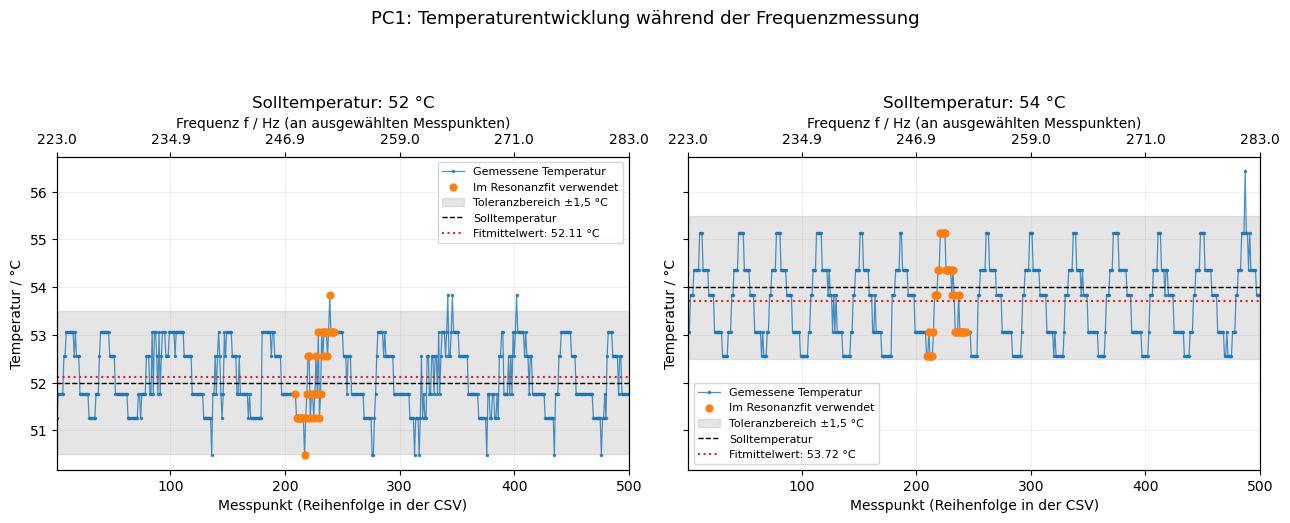
\includegraphics[width=0.95\linewidth]{T_plots/Tempentwicklung.png}
    \caption[PC1: Temperaturregelung im Resonanzbereich]{Repräsentative Illustration des Verhaltens der Temperaturregelung bei unterschiedlichen Werten für $\gamma$. Links eine Messung aus der ersten Nacht mit \(T_{\text{soll}}=\qty{52}{\degreeCelsius}\) und \(\gamma=1.1\), rechts eine Messung aus der zweiten Nacht bei \(T_{\text{soll}}=\qty{54}{\degreeCelsius}\) und \(\gamma=1.05\). Im späteren Fit für die Resonanz wurden nur die orange markierten Messpunkte verwendet, da im übrigen Frequenzbereich lediglich der Untergrund aufgezeichnet wurde.}
    \label{fig:TempReg-behave}
\end{figure}
\FloatBarrier

\zcref{fig:PC1-T-upper,fig:PC1-T-lower} zeigen die Ergebnisse nach Fits von \zcref{eq:fit_amplitude} auf die Datenpunkte im Frequenzbereich zwischen 248 Hz und 252.2 Hz. In \zcref{fig:PC1-T-lower} ist unten rechts überdies die Temperaturabhängigkeit der Resonanz aufgetragen, mit einem linearen und Konstanten Fit. Für den linearen Fit wurden hierbei explizit die Unsicherheiten sowohl der Temperatur als auch der Eigenfrequenz berücksichtigt. Dazu wurde das Modell $f_0(T)=a(T-T_{\mathrm{ref}})+c$ mit $T_{\mathrm{ref}}=50\,^\circ\mathrm{C}$ verwendet und die zu minimierende Größe
\begin{equation}
    \chi^2(a,c)=\sum_{i=1}^{N}
    \frac{\left[f_{0,i}-a(T_i-T_{\mathrm{ref}})-c\right]^2}
    {\sigma_{f_0,i}^2+a^2\sigma_{T,i}^2}
\end{equation}
definiert. Die Unsicherheit der Temperatur geht dabei über die Fehlerfortpflanzung mit dem Faktor $a^2$ in die effektive Varianz ein. Als Temperaturunsicherheit $\sigma_{T,i}$ wurde jeweils die Stichprobenstandardabweichung der während des Resonanzfits berücksichtigten Temperaturmesswerte verwendet, während $\sigma_{f_0,i}$ aus der Unsicherheit des jeweiligen Resonanzfits stammt. Die Unsicherheiten der Fitparameter $a$ und $c$ wurden aus der inversen Krümmungsmatrix von $\chi^2/2$ am Minimum bestimmt, wobei die Korrelation zwischen beiden Parametern berücksichtigt wurde. Das in \zcref{fig:PC1-T-lower} dargestellte $1\sigma$-Unsicherheitsband ergibt sich durch entsprechende Fehlerfortpflanzung unter Verwendung dieser Kovarianzmatrix. Der konstante Fit wird aus dem mit den inversen Varianzen $1/\sigma_{f_0,i}^2$ gewichteten Mittelwert der $f_0$-Werte berechnet, also $c=\sum_i f_{0,i}/\sigma_{f_0,i}^2\,/\,\sum_i 1/\sigma_{f_0,i}^2$. Seine Unsicherheit ergibt sich unter Annahme unabhängiger Messfehler durch Fehlerfortpflanzung zu $\sigma_c=\left(\sum_i 1/\sigma_{f_0,i}^2\right)^{-1/2}$.

\begin{figure}
    \centering
    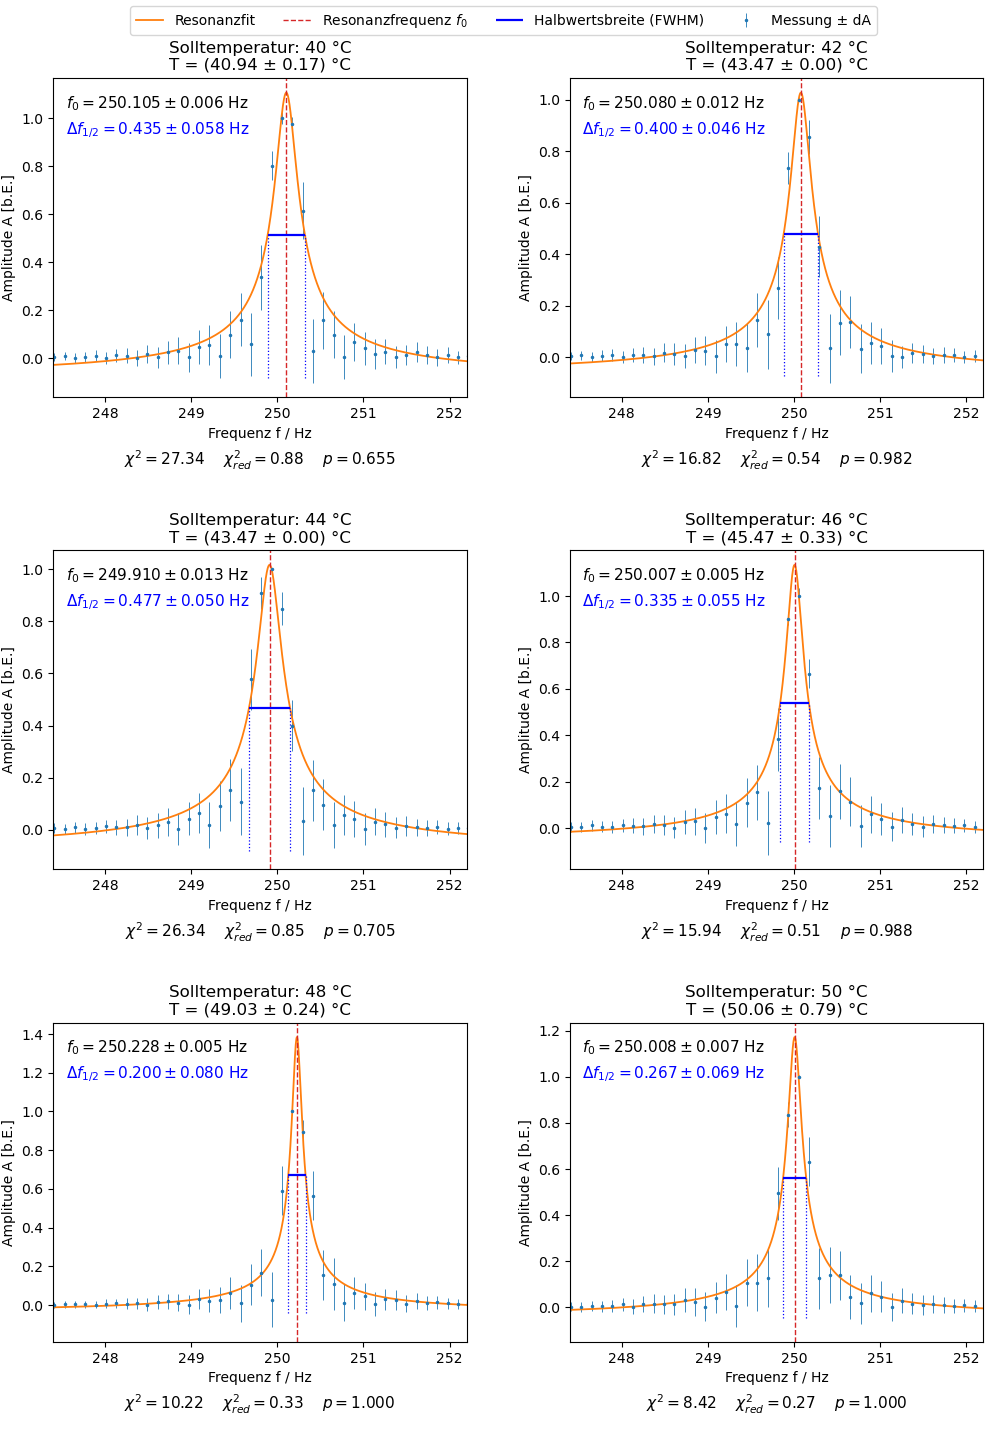
\includegraphics[width=0.9\linewidth]{T_plots/PC1 Temps upper part.png}
    \caption[PC1: Resonanzkurven (niedrige Temperaturen)]{PC1: nullte Mode bei verschiedenen Temperaturen (Mode \(n=0\))für den unteren Temperaturbereich - oben Solltemperatur, darunter tatsächlicher Temperaturmittelwert der für den Fit verwendeten Darenpunkte. In den Abbildungen: Aus Fitparametern berechnete Eigenfrequenz \(f_0\) und Halbwertsbreite \(\Delta f_{1/2}\). Darunter \(\chi^2\)-Summe des Fits neben reduzierter \(\chi^2\)-Summe \(\chi^2_{red}\) und Fitwahrscheinlichkeit $p$.}
    \label{fig:PC1-T-upper}
\end{figure}
\FloatBarrier

\begin{figure}
    \centering
    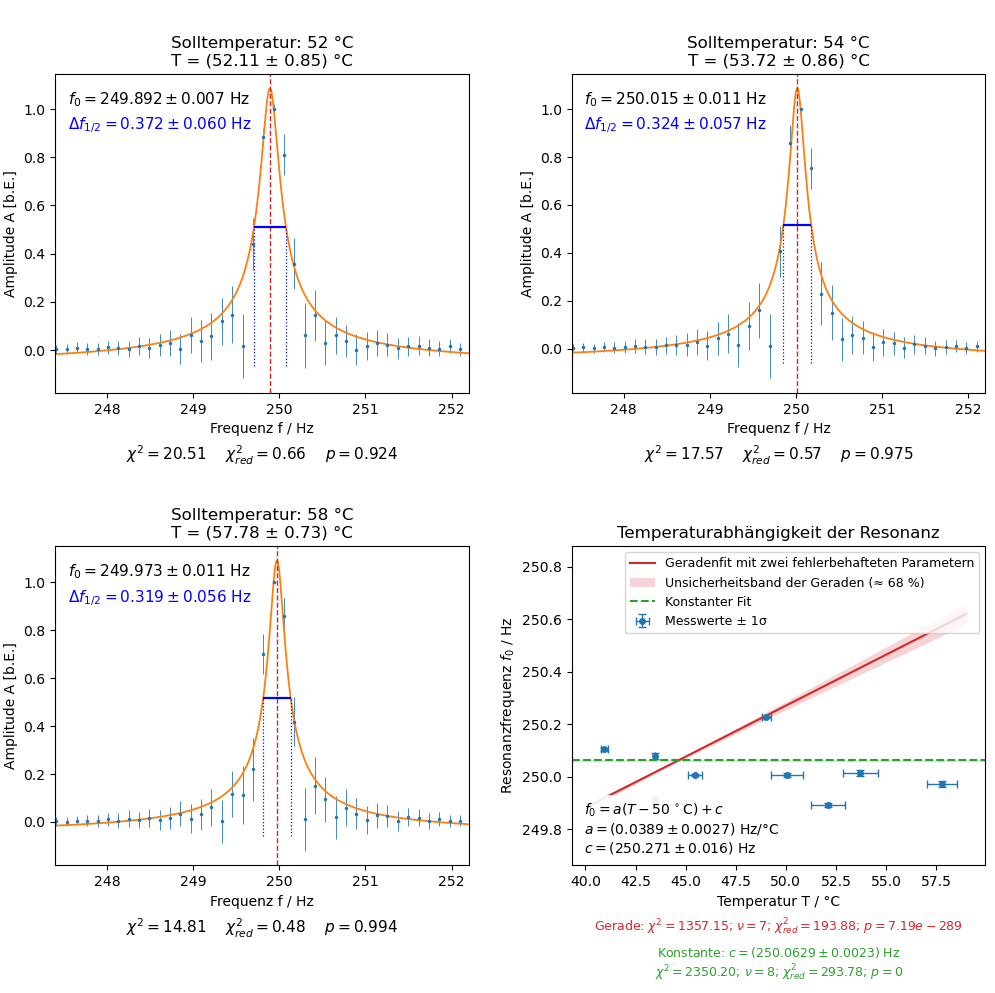
\includegraphics[width=0.97\linewidth]{T_plots/PC1 Temps lower part.png}
    \caption[PC1: Resonanzkurven (hohe Temperaturen) und Temperaturabhängigkeit]{Mode \(\nu=0\) bei PC1 für den oberen Temperaturbereich - sämtliche Werte wie \zcref{fig:PC1-T-upper}. Unten rechts: Per Fit ermittelte Eigenfrequenzen gegen die Temperatur (Durchschnittswert der verwendeten Daten mit Standardabweichung als Unsicherheit) aufgetragen, dazu linearer (rot) uns Konstanter Fit (grün) mit optimalen Parametern und entsprechenden Werten für \(\chi^2\), \(\chi^2_{red}\) und Fitwahrscheinlichkeit \(p\).}
    \label{fig:PC1-T-lower}
\end{figure}
\FloatBarrier

Insgesamt sind sowohl der Konstante, als auch der Lineare Fit extrem unwahrscheinlich, was die Abhängigkeit der Resonanzfrequenzen von der Temperatur nicht klar beschreibbar macht. Auch ob die Resonanzfrequenzen mit zunehmender Temperatur steigen oder sinken, lässt sich aufgrund der hohen Fitunsicherheit hieraus nicht klar folgern. Aus diesem Grund wurde im folgenden Teil noch die Korellation zwischen Temperatur und Resonanzfrequenzen berechnet, unter Verwendung von Monte-Carlo Sampling, um die Unsicherheiten korrekt miteinzubeziehen. 

\textbf{Berechnung des Pearson-Korrelationskoeffizienten}

Für die Berechnung des Korrelationskoeffizienten wurde Monte-Carlo-Sampling mit $10^5$ Iterationen durchgeführt.  Hierzu wurden für jeden Messpunkt normalverteilte Zufallswerte entsprechend den gemessenen Werten und ihren jeweiligen Unsicherheiten erzeugt und für jede Stichprobe der Korrelationskoeffizient bestimmt. Hiermit erhält man für die Korrelation $r_{MC}$:
\begin{equation}
    \boxed{r_{\mathrm{MC}}=-0{,}257^{+0{,}042}_{-0{,}041}}
\end{equation}
wobei die angegebenen Unsicherheiten das zentrale $68\,\%$-Intervall der simulierten Korrelationskoeffizienten beschreiben. Das entsprechende $95\,\%$-Intervall beträgt $[-0{,}336;\,-0{,}174]$. Damit zeigen die Messwerte eine schwache negative lineare Korrelation, also eine Tendenz zu sinkenden Eigenfrequenzen bei steigender Temperatur - also ein gegensätzliches Resultat im Vergleich zum linearen Fit, der auf eine positive Steigung von $a=(0{,}0389\pm0{,}0027)\,\mathrm{Hz}/^\circ\mathrm{C}$ führte.



\subsubsection{Temperaturabhängigkeit bei PC2}

Mit demselben Temperaturregelungsalgorithmus wie bei PC1 (\(\gamma=1.05\) wurden für PC2 Resonanzkurven der nullten Mode \(n=0\) im Bereich zwischen 160 Hz und 400 Hz aufgenommen. Die Messungen erfolgten am Nachmittag am vom 7. August 2026 bei Solltemperaturen von 37, 40, 43, 46, 49, 52, 55 und 58 \(^\circ\)C. Zur Untersuchung des Verhaltens der Temperaturregelung zeigt \zcref{fig:PC2_temp_development} das Verhalten der gemessenen Temperatur im Verlauf der Messungen (die x-Achse entspricht der Frequenz des bei dieser Temperatur aufgenommenen Messpunkts). Die Farben zeigen die jeweilige Solltemperatur. 


\begin{figure}[htbp]
\centering
    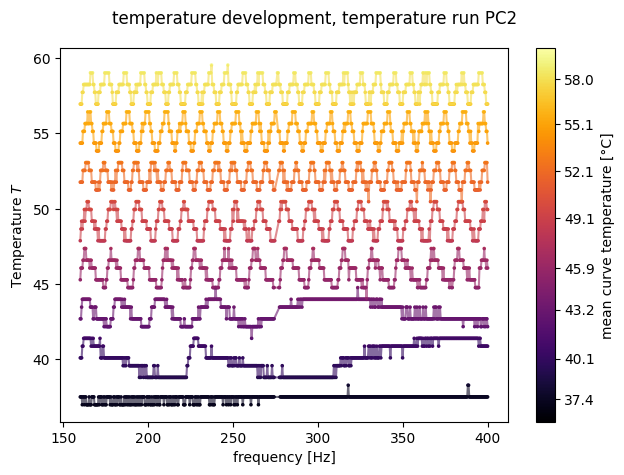
\includegraphics[width=0.6\textwidth]{figures/PC2/Plot_temp_development_final_TempFreq.png}
    \caption{PC2: Entwicklung der Temperatur}
    \label{fig:PC2_temp_development}
\end{figure}
\FloatBarrier


In \zcref{fig:PC2-T-grey} sind die Daten gemeinsam mit Fits (dabei wurden wie zuvor die Messwerte, bei denen X oder Y in Sättigung lagen, ignoriert) und denselben Kenndaten wie für PC1 dargestellt. 

\clearpage

\begin{figure}
    \centering
    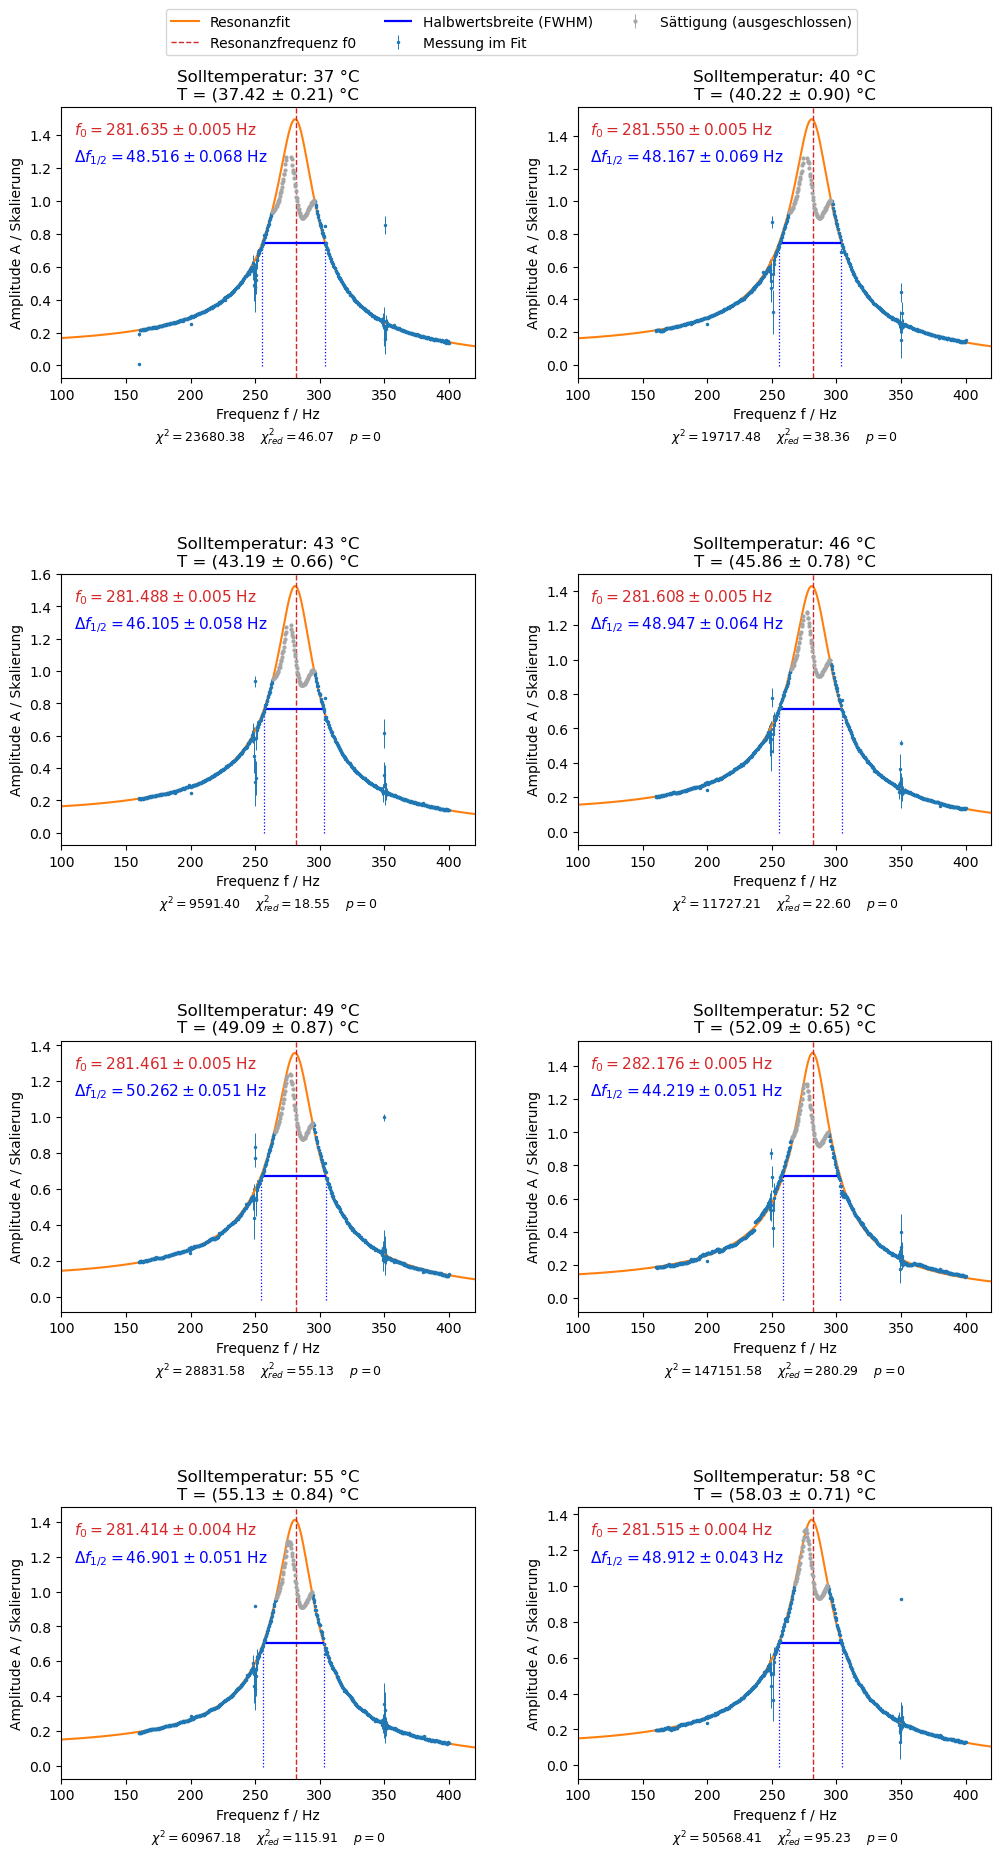
\includegraphics[width=0.75\linewidth]{T_plots/PC2 Temps greyed.png}
    \caption[PC2: Resonanzkurven bei variierten Temperaturen]{PC2: nullte Mode bei verschiedenen Temperaturen (Mode \(n=0\)) - oben Solltemperatur, darunter tatsächlicher Temperaturmittelwert der für den Fit verwendeten Darenpunkte. Ausgegraute Datenpunkte wurden wie zuvor aufgrund der Sättigung von X oder Y ausgeschlossen und nicht in den Fit mit einbezogen. In den Abbildungen: Aus Fitparametern berechnete Eigenfrequenz \(f_0\) und Halbwertsbreite \(\Delta f_{1/2}\). Darunter \(\chi^2\)-Summe des Fits neben reduzierter \(\chi^2\)-Summe \(\chi^2_{red}\) und Fitwahrscheinlichkeit $p$.}
    \label{fig:PC2-T-grey}
\end{figure}
\FloatBarrier
\clearpage

Wie für PC1 wurden auch für PC1 ein beidseitig mit Unsicherheiten behafteter linearer Fit und ein konstanter Fit durchgeführt, die gemeinsam mit den optimalen Parametern in \zcref{fig:PC2-line-grey} aufgetragen sind. Die Fitwahrscheinlichkeit ist jedoch wie zuvor verschwindend gering und der \(\chi^2_{red}\)-Wert von \(\chi^2_{red}\approx250\) ist sogar größer als bei den Daten von PC1 (dort hatten wir \(\chi^2_{red}\approx 190\)). 

\begin{figure}[htbp]
    \centering
    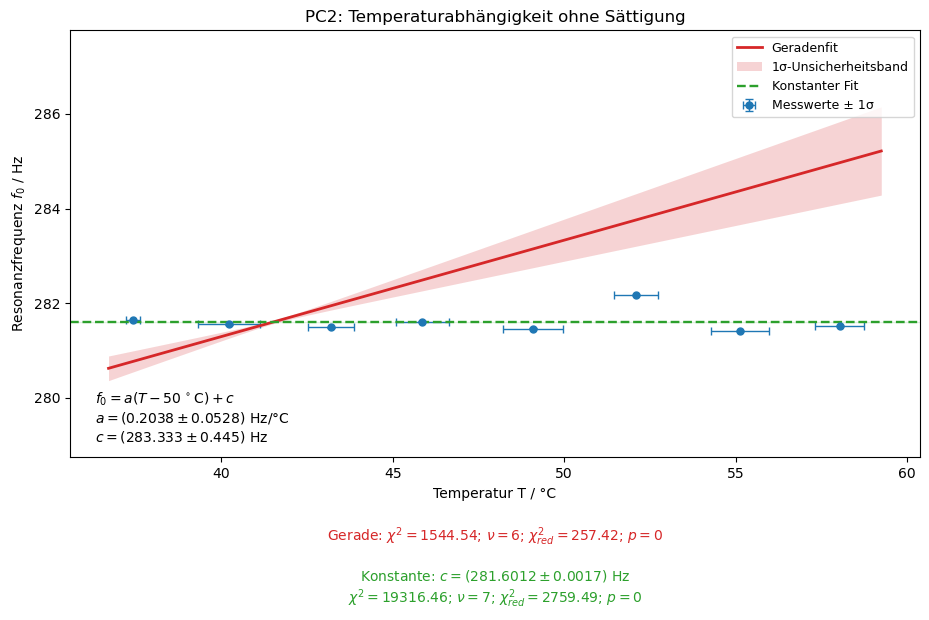
\includegraphics[width=0.75\linewidth]{T_plots/PC2 linear fit grey.png}
    \caption[PC2: Temperaturabhängigkeit der Resonanzfrequenzen]{PC2: Per Fit ermittelte \(f_0\) gegen Temperaturen aufgetragen. Unsicherheiten wie zuvor aus Fitunsicherheit und Standardabweichung der verwendeten Datenpunkte. Rot: linearer Fit mit Unsicherheiten auf X- und Y-Achse. Grün: entsprechender konstanter Fit.}
    \label{fig:PC2-line-grey}
\end{figure}

Aufgrund schlechten Fitwahrscheinlichkeiten wurde wieder der Pearson-Korellationskoeffizient berechnet, mit dem Ergebnis:

\begin{equation}
    \boxed{r_{\mathrm{MC}}=0{,}048^{+0{,}036}_{-0{,}036}}
\end{equation}

Dieser liegt für PC2 also deutlich näher an Null und ist im Gegensatz zu PC1 positiv. Damit zeigt er zwar in dieselbe Richtung wie die ermittelte Geradensteigung \(a=0.20 \pm 0.05\) Hz/\(^\circ\)C, insgesamt spricht man bei so nahe an Null liegenden Korrelationswerten aber nicht von positiver Korrelation.

\section{Diskussion}

Im nachfolgenden Teil diskutieren wir die unterschiedlichen Messergebnisse und bewerten die angewandten Methoden, insbesondere auch in Bezug auf die Programmierung für die automatisierten Messungen.

\subsection{Analyse der Implementierungsentscheidungen}
Die folgenden Entscheidungen in Bezug auf die Umsetzung der Automatisierung waren nicht trivial und werden im folgenden diskutiert. 
\paragraph{logarithmische Auflösung:} Das Frequenzintervall um eine bestimmte Resonanzfrequenz wurde mithilfe einer über das ganze Intervall konstanten Stepsize aufgenommen. Die genutzte python-libary \libary{numpy} bietet neben \verb|np.linspace| jedoch auch \verb|np.geomspace|, mit der sich logarithmisch abfallende Stepsizes um die Resonanzfrequenz implementieren ließen, sodass der Resonanzpeak am besten aufgelöst wird und die AUflösungsrate symmetrisch um die Resonanz logarithmisch kleiner eingestellt wurde. Dieses Vorgehen wurde aufgrund der sehr kleinen FHWM an PC1 verworfen, denn die logarithmische Aufteilung erfordert eine genaue Kenntnis von \(\nu_i\). Die FHWM an PC2 ist im Gegensatz so hoch, dass der Nutzen einer logarithmischen Auflösung als irrelevant eingeschätzt wurde. 

\paragraph{Zeitmessung:} Erst für die finalen PC2 Messungen wurde mithilfe der \libary{time.perf_counter} libary die pro Mode/Temperaturmessung vergangene Zeit erhoben und laufend in einer Datei gespeichert. Perspektivisch lohnt sich diese Implementierung für eine genauere Abschätzung der Nachtmessungszeit aufgrund von Testläufen, sowie die Detektion von Softwarefehlern, die die Messzeit ungewöhnlich erhöhen. In den vorliegenden Messungen zeigt sich: Die drei Resonanzmoden benötigten alle \(\qty{36}{\min}\), die Temperaturmessungen wurden durch eine mit der Temperatur steigenden, komplizierteren Regelung zeitintensiver: von \(\qtyrange{36}{100}{\min}\) bei \(\qty{58}{\degreeCelsius}\). Mithilfe der \libary{datetime} libary konnten laufend die aktuellen Start- und Enduhrzeiten eines einzelnen Messzykluses erhoben werden. Diese Daten wurden sowohl in der Zeitdatei gespeichert, und bilden damit im Nachhinein die Historie des Messaufbaus ab und können zur Evaluation der Aktivität des Messaufbaus genutzt werden. 

\paragraph{Emails:} Um eine wenigstens ansatzweises remote-controlling der Messungen zu ermöglichen, wurden der aktuelle Status (z.B.\ Mode 0) sowie deren jeweiligen Uhrzeiten und Dauern die gesamte Tag-/Nachmessung hinweg per Email an die Experimentatoren weitergeleitet. Dies funktioniert durch das Aufsetzen eines lokalen Emailservers durch die libary \libary{smtplib} und die Sendecommands von \libary{email.message}. Diese Funktion war sehr hilfreich, da im vorliegenden Fall die meisten Messungen tagsüber gestartet wurden, sodass während einer laufenden Messung anderen Beschäftigungen nachgegangen werden konnte, und dennoch im Notfall eingreifen zu können. Somit wurde z.B.\ beobachtet, dass in einer Messinstanz die einzelnen Frequenztupel aufgrund einer unscheinbaren, nicht entfernten Codezeile \(\qty{240}{\min}\) dauerten. Zudem konnte somit eine nicht startende Temperaturmessung aus der Ferne detektiert und daraufhin angepasst werden, die aufgrund leichtsinnig manuell eingestellter Temperatur \(T\) des Temperaturmessungsintervall (\(\approx \text{Raumtemperatur}\)) überhaupt nicht startete. In diesem Fall war die Soll-Temp.\ kleiner als die minimal regelbare Ist-Temp.\ des Reeds, wodurch der Temperaturregler die Messung nicht freigegeben hat. Daraufhin wurde das Problem behoben, indem die Starttemperatur automatisch auf die aufgerundete aktuelle Reedtemperatur gesetzt wird. 

Zudem war es durch den Emails angefügten Zeiten möglich, die Dauer der Messung deutlich besser zu verfolgen und abschätzen zu können. Neben der Benachrichtigung über den Abschluss der gesamten Messung, die zur Abholung der Messdaten tagsüber wichtig ist, konnte zudem durch eine entsprechende Email überprüft werden, dass die Spannung des Peltierelements und die Temperatur des Reeds zurückgesetzt wurden. Somit wurde erfolgreich eine konkrete Sicherheitsvorgabe in eine überprüfbare Maßnahme umgewandelt. 


\paragraph{Temperaturregelung}
Die nachträgliche Betrachtung der Temperaturverläufe zeigt, dass die implementierte Regelung zwar grundsätzlich funktionierte, jedoch häufig zu einem Überschwingen führte. Typischerweise wurde das Reed zunächst zu stark erhitzt, woraufhin die Heizspannung reduziert wurde und das System durch Wärmeabgabe an die Umgebung selbstständig abkühlte. Während dieser Abkühlphase lag die Temperatur vorübergehend innerhalb des gewünschten Toleranzbereichs. Unterschritt sie anschließend die untere Grenze, wurde erneut nachgeheizt, wobei die Regelung häufig wieder über das Ziel hinausschoss. Der Hauptgrund hierfür dürfte die thermische Trägheit des Aufbaus sein: Nach einer Spannungsänderung benötigt die Temperatur einige Zeit, um sich dem neuen Gleichgewichtswert anzunähern. Die im Programm vorgesehenen Wartezeiten von wenigen Sekunden waren hierfür offenbar zu kurz, sodass der Regler teilweise bereits weitere Korrekturen vornahm, bevor die vorherige Änderung ihre vollständige Wirkung entfalten konnte.

Dies erklärt auch plausibel die Unterschiede zwischen den beiden PC1-Messnächten in \zcref{fig:TempReg-behave}. Mit dem ursprünglichen Faktor $\gamma=1{,}1$ aus \zcref{eq:eta-update} vergrößerte sich die Schrittweite bei wiederholten Korrekturen in dieselbe Richtung schneller als mit dem später verwendeten Wert $\gamma=1{,}05$. Dadurch konnten bei verzögerter Temperaturreaktion größere Spannungsänderungen und entsprechend stärkere Überschwinger auftreten. Der kleinere Faktor führte zu einem sichtbar stabileren Regelverhalten, auch wenn andere Einflüsse auf den Vergleich der beiden Messnächte nicht vollständig ausgeschlossen werden können.

Bei PC2 ist überdies in \zcref{fig:PC2_temp_development} erkennbar, dass die Temperatur bei niedrigeren Sollwerten weniger stark schwankt. Dies ist plausibel, da diese Temperaturen näher an der während des Versuchs herrschenden Umgebungstemperatur von etwa $\qty{37}{\degreeCelsius}$ lagen. Hier dürfte teilweise bereits eine geringe Heizspannung genügt haben, um die Temperatur annähernd konstant zu halten. Gleichzeitig ist bei kleiner Temperaturdifferenz zur Umgebung die passive Abkühlung langsamer. Bei höheren Temperaturen führen größere Wärmeverluste dagegen zu einem stärkeren Regelbedarf, wodurch die verzögerte Reaktion des Systems und das damit verbundene Überschwingen deutlicher hervortreten.

Rückblickend wäre daher insbesondere eine deutlich längere Wartezeit nach jeder Änderung der Heizspannung sinnvoll gewesen. Alternativ wäre ein passend abgestimmter PI- oder PID-Regler denkbar, der die zeitliche Entwicklung der Temperatur expliziter berücksichtigt. Eine klassisch aufgestellte PI/D Regelung der Temperatur, insbesondere beim vorliegenden Reed, weist jedoch das Problem der Zeitlatenz/Trägheit zwischen Regelung und Auswirkung/Reaktion des Systems auf, wodurch das einfache Aufstellen einer PID-Regelung zu Probleme führen würde. Insgesamt hat die implementierte Regelung ihren Zweck dennoch erfüllt: Die Temperatur blieb während der eigentlichen Messungen weitgehend innerhalb des vorgegebenen Bereichs von $T_{\mathrm{soll}}\pm\qty{1.5}{\degreeCelsius}$, und der Abbruch der Regelung nach 100 erfolglosen Korrekturen trat nach unseren Beobachtungen kaum auf. Die Temperaturregelung war somit nicht besonders effizient, ermöglichte aber die weitgehend selbstständige Aufnahme vollständiger Resonanzkurven.

Eine weitere (ungeklärte) Beobachtung sind die teilweise über mehrere Messpunkte identischen Temperaturwerte, in \zcref{fig:PC2_temp_development} als diskrete Stufenform der Temperaturentwicklung zu sehen. Dies könnte auf die begrenzte Auflösung des Thermometers beziehungsweise die Quantisierung der aufgezeichneten Werte hindeuten: Das Pt-100 Thermometer muss eine bei mehreren Punkten und damit über mehrere Sekunden numerisch exakt gleiche Spannung zurückgeben haben, damit die gemappte und in der \verb|.csv| aufgezeichnete Temperatur \(T(U)\) konstant bleibt. Dieses Vorgehen zeigt sich in der konsistenten periodischen Abkühlung in \zcref{fig:PC2_temp_development}. Eine entsprechend kleine Stichprobenstandardabweichung bedeutet deshalb nicht zwangsläufig, dass die tatsächliche Temperatur des Reeds mit derselben Genauigkeit bekannt ist. Zudem können thermische Gradienten zwischen Temperatursensor und Reed auftreten, die in der verwendeten Temperaturunsicherheit nicht berücksichtigt werden.



\subsection{Zusammenfassung der Ergebnisse}


In Versuchsabschnitt A konnten bei beiden Aufbauten Schwingungsmoden in den erwarteten Frequenzbereichen identifiziert werden. Während PC2 für alle drei untersuchten Moden auswertbare Resonanzkurven lieferte, waren die Ergebnisse von PC1 insbesondere bei höheren Moden durch starke Schwankungen und teilweise nicht auflösbare Resonanzspitzen eingeschränkt. Besonders auffällig war die stark unterschiedliche Güte der beiden Aufbauten: Für die nullte Mode wurde bei PC1 $Q_0=\num{1150(40)}$ bestimmt, während sich bei PC2 $Q_0=\num{10.629(0.015)}$ ergab. Damit unterscheiden sich die Güten um mehr als zwei Größenordnungen.

In Versuchsabschnitt B konnten bei beiden PCs automatisierte Resonanzmessungen über einen Temperaturbereich von ungefähr $\qtyrange{37}{58}{\degreeCelsius}$ durchgeführt werden (bzw.\ von aktuell bestimmter Raumtemperatur bis \(\qty{58}{\degreeCelsius}\), eine manuell eingestellte Temperatur könnte oberhalb der niedrigsten Reedtemperatur liegen - ohne aktive Kühlung wäre eine Messung dann unmöglich). Die Untersuchung der Temperaturabhängigkeit ergab jedoch keinen eindeutig beschreibbaren linearen Zusammenhang, da sowohl die linearen als auch die konstanten Fits sehr große reduzierte $\chi^2$-Werte aufwiesen. Die ergänzende Korrelationsanalyse lieferte bei PC1 eine schwache negative Korrelation von $r_{\mathrm{MC}}\approx-0{,}257$, bei PC2 dagegen einen nahezu verschwindenden Zusammenhang mit $r_{\mathrm{MC}}\approx0{,}048$. Die physikalische Interpretation dieser Ergebnisse wird durch die systematischen Messabweichungen und die unvollständig erfassten Unsicherheiten eingeschränkt.


\subsection{Bewertung der Fits}

\paragraph{Fitqualität und Messunsicherheiten}
Die Qualität der Resonanzfits unterscheidet sich zwischen den beiden Aufbauten erheblich. Bereits in Versuchsabschnitt A lag bei PC1 für die nullte Mode ein reduziertes $\chi^2_{\mathrm{red}}\approx4{,}6$ vor, während die entsprechenden Werte bei PC2 für die drei untersuchten Moden wesentlich größer waren. In Versuchsabschnitt B dagegen ergaben sich bei PC1 für die einzelnen Resonanzkurven überwiegend reduzierte $\chi^2$-Werte unter eins. Bei PC2 lagen diese selbst nach dem Ausschluss gesättigter Messwerte teilweise noch bei mehreren Hundert, mit einem besonders hohen Wert von $\chi^2_{\mathrm{red}}\approx280$ bei der Solltemperatur von $\qty{52}{\degreeCelsius}$. Ein eindeutiger monotoner Zusammenhang zwischen Temperatur und Fitqualität ist hierbei nicht erkennbar.

Insgesamt dürfte die wesentliche Ursache der großen $\chi^2$-Werte in der Unterschätzung der tatsächlichen Messunsicherheiten liegen. Die verwendeten Amplitudenfehler wurden aus wiederholten Messungen bei festgehaltener Frequenz bestimmt und beschreiben damit vor allem kurzfristige statistische Schwankungen. Längerfristige Drifts, Veränderungen der Anregungsbedingungen oder systematische Abweichungen vom theoretischen Modell werden dadurch nicht zwangsläufig erfasst. Gerade bei PC2 waren die statistischen Fehler sehr klein, sodass bereits geringe systematische Unterschiede zwischen Fitkurve und Messpunkten zu großen normierten Residuen führen konnten.
Bei PC1 dagegen schwankte die Anzeige des im unmittelbaren Resonanzbereich teilweise sehr stark, wodurch größere statistische Fehler entstanden, dies kann erklären, weshalb die einzelnen Resonanzfits dort trotz augenfälliger Unregelmäßigkeiten teilweise reduzierte $\chi^2$-Werte unter eins aufweisen.

\paragraph{Systematische Abweichungen bei PC2}
Bei PC2 stellte die Sättigung der Quadraturkomponenten $X$ und $Y$ eine zusätzliche Fehlerquelle dar. Da die beiden Komponenten bei unterschiedlichen Frequenzen ihre Sättigungsgrenzen erreichten, wurde die daraus berechnete Amplitude $A=\sqrt{X^2+Y^2}$ künstlich verformt, sodass teilweise ein scheinbarer Doppelpeak entstand. Die als gesättigt identifizierten Messpunkte wurden deshalb vom Resonanzfit ausgeschlossen und in den Diagrammen grau dargestellt. Dieser Ausschluss verbesserte die Beschreibung der Resonanzkurven durch das theoretische Modell, beseitigte die systematischen Abweichungen jedoch nicht vollständig.

Insbesondere treten bei mehreren Messungen in der Nähe von $\qty{250}{\hertz}$ und $\qty{350}{\hertz}$ auffällige Abweichungen vom ansonsten glatten Resonanzverlauf auf. Diese Punkte wurden ausdrücklich nicht ausgeschlossen und tragen somit weiterhin zu den hohen $\chi^2$-Werten bei. Ihre wiederholte Lage bei ungefähr denselben Frequenzen spricht für einen instrumentellen Einfluss. Denkbar wären etwa Störungen durch eingekoppelte Netzspannung beziehungsweise deren Oberwellen, da beide Bereiche in der Nähe ganzzahliger Vielfacher von $\qty{50}{\hertz}$ liegen. Ein solcher Zusammenhang lässt sich mit den vorhandenen Daten jedoch nicht nachweisen. Ebenso kommen frequenzabhängige Eigenschaften der Messelektronik oder weitere mechanische Schwingungsbeiträge infrage. In der Versuchsanleitung werden unter anderem elektronische Störungen, mechanische Fehlerquellen und Abweichungen von den idealisierten Modellannahmen diskutiert \autocite[24--25]{Skript}.

\paragraph{Unterschiede zwischen PC1 und PC2}
Die stark unterschiedlichen Güten der beiden Aufbauten lassen sich aus den verfügbaren Informationen nicht eindeutig erklären. Bei PC1 wurde für die nullte Mode eine Güte von ungefähr $Q_0=1150$ bestimmt, während sie bei PC2 nur etwa $Q_0=10{,}6$ betrug. Die deutlich schmalere Resonanz von PC1 weist somit auf eine wesentlich geringere relative Dämpfung hin. Eine mögliche Erklärung liegt in Unterschieden der mechanischen Einspannung, da die größten mechanischen Verzerrungen des Reeds gerade an der Einspannstelle auftreten. Bereits geringfügige Unterschiede der Kontaktbedingungen könnten deshalb zu unterschiedlichen Energieverlusten führen. Daneben kommen unterschiedliche Materialeigenschaften, geometrische Abmessungen oder zusätzliche Dämpfungsmechanismen infrage. Da die Reeds selbst nicht sichtbar waren und die äußerlich nahezu identischen Aufbauten nicht geöffnet werden durften, kann keine dieser Erklärungen überprüft werden. Die stark unterschiedlichen Resonanzkurven müssen daher als experimenteller Befund mit ungeklärter Ursache festgehalten werden.

\paragraph{Temperaturabhängigkeit und Korrelationsanalyse}
Auch die Fits zur Temperaturabhängigkeit weisen erhebliche Probleme auf. Bei PC1 ergab sich für die lineare Regression ein reduziertes $\chi^2_{\mathrm{red}}\approx194$, während der konstante Fit mit $\chi^2_{\mathrm{red}}\approx294$ noch schlechter abschnitt. Bei PC2 lagen die entsprechenden Werte ebenfalls weit oberhalb von eins. Somit beschreibt weder das lineare noch das konstante Modell die beobachteten Frequenzwerte innerhalb der angesetzten Unsicherheiten ausreichend gut.

Ein Problem des verwendeten linearen Fitverfahrens besteht darin, dass die effektive Varianz im Nenner der $\chi^2$-Summe selbst von der gesuchten Steigung $a$ abhängt, nämlich über den Term $a^2\sigma_{T,i}^2$. Bei großen Temperaturunsicherheiten kann dadurch eine betragsmäßig größere Steigung die $\chi^2$-Summe reduzieren, weil gleichzeitig die Gewichtung der Residuen verringert wird. Dieses Verfahren entspricht damit nicht einer gewöhnlichen linearen Regression mit festen Gewichten und kann unter den vorliegenden Bedingungen Steigungen begünstigen, die den augenfälligen Trend der Messpunkte nur schlecht wiedergeben. Die resultierenden sehr kleinen formalen Parameterfehler dürfen angesichts der erheblichen Modellabweichungen daher nicht als verlässlicher Nachweis einer Temperaturabhängigkeit interpretiert werden.

Zur ergänzenden Untersuchung wurde deshalb der Pearson-Korrelationskoeffizient herangezogen, der alle Messpunkte gleich gewichtet und keine von der Steigung abhängige Fehlervarianz verwendet. Seine Empfindlichkeit gegenüber den angenommenen Messunsicherheiten wurde mittels Monte-Carlo-Sampling mit $10^5$ Iterationen bestimmt. Für PC1 ergab sich eine schwache negative Korrelation von $r_{\mathrm{MC}}\approx-0{,}257$, während PC2 mit $r_{\mathrm{MC}}\approx0{,}048$ praktisch keinen linearen Zusammenhang zeigte. Insbesondere bei PC1 steht das negative Vorzeichen im Gegensatz zur positiven Steigung des linearen Fits. Der Korrelationskoeffizient beschreibt damit den beobachteten Trend anschaulicher, berücksichtigt jedoch selbst keine systematischen Messfehler. Auch das Monte-Carlo-Intervall erfasst nur die Auswirkungen der angenommenen Unsicherheiten und stellt kein Konfidenzintervall für eine zugrunde liegende physikalische Korrelation dar.

Das negative Vorzeichen bei PC1 wäre grundsätzlich mit einer thermisch bedingten Abnahme der Schwingungsfrequenz vereinbar. Für die Biegeschwingung gilt näherungsweise $\nu\propto(d/l^2)\sqrt{E/\rho}$, wobei $E$ den Elastizitätsmodul bezeichnet. Da dieser bei vielen Metallen mit zunehmender Temperatur abnimmt, wäre unter ansonsten gleichbleibenden Bedingungen ebenfalls eine sinkende Frequenz zu erwarten. Thermische Ausdehnung und mögliche Änderungen der Einspannbedingungen können diesen Zusammenhang zusätzlich beeinflussen. Die beobachtete negative Korrelation ist somit qualitativ plausibel, erlaubt aufgrund der großen systematischen Unsicherheiten und der unbekannten Materialeigenschaften jedoch keine quantitative Bestätigung der theoretischen Erwartung.

\subsection{potenzielle Fehlerursachen in der Messapparatur}
Das erwähnte Schwanken der LoVe-Anzeige bei PC1 ist eine weitere ungeklärte und besorgniserregende Beobachtung: Die Anzeigefelder (Nadelskala) des LoVe im Resonanzbereich haben bei einer eingestellten Frequenz! \emph{total am Rad gedreht}, die Nadeln schwangen sehr schnell von minimalen bis maximalen Ausschlag, daher kommt der hohe statistische Fehler im Bereich der Resonanz. Es wäre zu erwarten gewesen, dass die Amplitude bei einer eingestellten Frequenz konstant bleibt (abgesehen von einem minimalen Einstellvorgang). Das könnte eine Fehlfunktion des LoVe vermuten lassen. Bei PC2 (anderer LoVe) im Gegensatz sind nur sehr geringe statistische Fehler aufgenommen worden, da der LoVe konstante Amplituden ausgelesen hat.

Es können nur Vermutungen angestellt werden, welchen Ursprung diese \enquote{hässlichen} PC1 Messdaten haben: Dass die aufgezeichneten Kurven im Resonanzbereichs des Reeds auftreten, schließt eine kaputte Verbindung der Ausleseelektronik aus. Dennoch kann es sein, dass die Verschaltung und Kalibrierung der Aufbauten die existierenden Messdaten nicht optimal aufnimmt und verarbeitet. Dies ist schwierig zu beurteilen, da der Fokus des Versuchs nicht auf dem Verständnis, Einstellung und Überprüfung des Experimentieraufbaus bestand. Eine fehlerhafte Einstellung oder Fehlfunktion des LoVe kann auch für korrumpierte Signale veranwortlich sein. Alle im Skript erklärten Einstellungen wurden wie vorgegeben durchgeführt, neben einer Fehleinstellung aufgrund mangelnder Informationen kann auch menschliches Versagen für eine potenzielle Fehlfunktion des LoVe veranwortlich sein. Eine weitere Fehlerquelle kann eine inkonsistente Phase bei festem Frequenzwert durch Fehlfunktion des Frequenzgenerators sein. Dies könnte mittels eines Oszilloskops untersucht werden.

Ein grobes Fehlverhatlen des Codes in der Auslese kann ausgeschlossen werden, da dieser an zwei Aufbauten/PCs getestet wurde und zudem der Code einer anderen Gruppe auf PC1 lief, dieser zeigte ähnliche Messdaten.
Im Skript sind verschiedene Ursachen elektronischen Rauschens genannt, dass diese eine Resonanzkurve derart verfälschen, ist nicht zu vermuten. Die Unsicherheiten der PC2 Messdaten werden dahingegen wahrscheinlich hauptsächlich durch elektronisches Rauschen verursacht.

\subsection{Bewertung der Messstrategie und Programme}
Das Aufbauen des Messprogramms in modularer Kombination von Klassen hat sich als sehr sinnvolles Vorgehen erwiesen. Ein Learning liegt darin, konsistent einen Testmodus mit zu implementieren bzw.\ für die finalle Messzelle, die alle Klassenfunktionen zur Nachtmessung vereint, als eigene Klasse zu schreiben, um somit evtl.\ einfacher einen Testmodus der Nachtmessung einstellen zu können, der Sicherheit in der Funktionalität gibt. Denn es sind, mindestens einmal, durch Leichtsinnscodefehler Nachtmessungen gecrasht.

Für zukünftige Messungen wäre insbesondere eine größere Anzahl unterschiedlicher Temperaturen sinnvoll. Die vorliegenden acht beziehungsweise neun Temperaturmessungen reichen zwar aus, um einen möglichen Trend zu untersuchen, machen die Ergebnisse aber empfindlich gegenüber einzelnen auffälligen Messpunkten. Darüber hinaus sollte der bislang zulässige Temperaturbereich von $\pm\qty{1.5}{\degreeCelsius}$ deutlich verkleinert werden. Wichtiger als eine bloße Verringerung der Toleranz wäre jedoch eine tatsächliche thermische Stabilisierung vor Beginn der Messung. Beispielsweise könnte zusätzlich gefordert werden, dass die zeitliche Änderungsrate der Temperatur über ein längeres Intervall unterhalb eines vorgegebenen Grenzwertes liegt. Damit ließen sich systematische Temperaturänderungen während der Aufnahme einer Resonanzkurve zumindest verringern.

Bei PC1 wäre außerdem eine höhere Frequenzauflösung unmittelbar um die sehr schmalen Resonanzspitzen zweckmäßig gewesen. Ein zunächst grober Suchscan mit anschließender adaptiver Verfeinerung des Frequenzintervalls hätte vermutlich weniger Zeit benötigt als die Aufnahme ausgedehnter Bereiche mit sehr kleinen Frequenzschritten. Bei PC2 dagegen wäre vor allem eine zusätzliche Kontrolle des Messbereichs des Lock-In-Verstärkers sinnvoll gewesen, um die Sättigung der Quadraturkomponenten bereits während der Messung zu erkennen und nach Möglichkeit durch eine geeignete Verstärkungseinstellung zu vermeiden. Insgesamt wären weniger systematische Störungen, eine stabilere Temperaturregelung und eine bessere Anpassung der Messstrategie an den jeweiligen Aufbau voraussichtlich hilfreicher gewesen als eine weitere Erhöhung der Anzahl einzelner Frequenzmesspunkte.



\subsection{Fazit}
Bei der Auswertung der PC1 Daten traten zahlreiche Unstimmigkeiten auf, die es unmöglich machten,
aus den aufgezeichneten Daten nennenswerte physikalische Erkenntnisse zu gewinnen. Insgesamt gibt es
viele potenzielle Fehlerquellen, welche konkret veranwortlich sind, kann  allein auf der Grundlage der erfassten Daten nicht eindeutig festgestellt werden. Die Unstimmigkeiten bei den Resonanz- und Phasendaten von PC1, bedeuten, dass dieser Datensatz mit äußerster Vorsicht analysiert werden sollte und sich daraus nur wenig bis gar keine physikalischen
Aussagen ableiten lassen. 

Insgesamt war der Versuch insbesondere hinsichtlich der eigenständigen Programmierung, Automatisierung und statistischen Auswertung der Messungen lehrreich. Bedauerlich war jedoch, dass sich die beiden äußerlich nahezu identischen Aufbauten derart unterschiedlich verhielten und insbesondere das Auffinden der sehr schmalen Resonanzen bei PC1 erheblichen Zeitaufwand erforderte. Obwohl die physikalische Aussagekraft der Ergebnisse durch systematische Messabweichungen eingeschränkt blieb, konnte das wesentliche Versuchsziel einer weitgehend automatisierten Messdatenerfassung und anschließenden quantitativen Auswertung und Datenanalyse erreicht werden.


\printbibliography[heading=bibintoc,title={Literaturverzeichnis}]

\end{document}
